\part{Methodological aspects of probabilistic dynamic security assessment}
\label{part:PDSA}
\chapter{Probabilistic dynamic security assessment}
\label{ch:DPSA}
\minitoc

\begin{tcolorbox}[width=\linewidth, sharp corners=all,
    colback=white!80!black,
    colframe=white!80!black]
This chapter is partly based on the following publication:
\begin{itemize}
    \item \fullcite{Journal_paper}
\end{itemize}
\end{tcolorbox}

Thanks to the previous chapters, we are now able to list the contingencies that can affect power systems, estimate their frequency of occurrence, and, for any given initial system state, estimate the potential consequences of these contingencies. The last remaining block to build a probabilistic dynamic security assessment (PDSA) methodology is the estimation of some form of probability density function (pdf) of the initial system states. Fortunately, this has been studied extensively in the literature that is reviewed in section~\ref{sec:operating_conditions}.

With all main building blocks available, it is then possible to develop a coherent PDSA methodology which is the focus of section~\ref{sec:PDSA_methodology}. This methodology is then applied to a standard test system (described in section~\ref{sec:PDSA_test_system}) in section~\ref{sec:PDSA_results}.

Probabilistic methodologies require numerous simulations which renders the interpretation of results more complex than with deterministic assessments. Some methods to interpret the results of PDSAs are thus presented in section~\ref{sec:PDSA_interpretation}. Probabilistic methodologies are intrinsically more complex than deterministic ones. To justify the need for this higher complexity, the added value of using probabilistic methods is discussed in section~\ref{sec:cascade_value}. Also, probabilistic methods require to perform many simulations which implies high computation times. The scalability of the methodology to large grids is thus discussed in section~\ref{sec:PDSA_scalability}. Finally, section~\ref{sec:PDSA_conclusion} concludes with a summary and perspectives.

\section{Operating conditions}
\label{sec:operating_conditions}

Two main methodologies have been developed in the literature to approximate the true pdf of the operating conditions of power systems.

The first methodology has initially been developed during the GARPUR (Generally Accepted Reliability Principle with Uncertainty modelling and through probabilistic Risk assessment) project~\cite{StrathElia, StrathGARPUR} and is now used by some European TSOs and by ENTSO-E to perform adequacy studies~\cite{ACER_MC_year, EliaAdequacy, ENTSOE_MC_year}. This methodology uses weather data (historical data and climate predictions) to build so-called ``Monte Carlo (MC) years''. These MC years are time-series realisations of temperature-dependent load, wind and solar availability, hydro inflows (rain, ice melting) and random availability (due to forced outages) of generating units and transmission elements. The use of weather data allows for adequate modelling of the spatio-temporal correlations between all random variables (renewable availability, load, asset availability)~\cite{StrathGARPUR, ENTSOE_MC_year}. Then, for each MC year, a market model is used to determine the commitment of thermal and hydro generators. Finally, each year is divided into (\eg hourly) snapshots and an optimal power flow (OPF) is performed to account for potential preventive actions that could be performed by operators to make the system secure. Typically, this OPF will include constraints to guarantee that static limits are not exceeded in all possible N-1 conditions. All snapshots are then saved in a database to be used in the rest of the analysis (\eg adequacy or security assessment\footnote{Depending on the type of analysis, a different level of granularity might be used. For adequacy studies, a zonal approach is typically used, while for security studies, a nodal approach is used.}).


The second methodology has been developed during the iTesla project~\cite{KonstantelosCopulas, EurostagHPC, iTesla_uncertainties}. It consists in directly fitting a multivariate pdf to the true pdf of system states using historical data. Copulas are used to model the correlations between variables. The advantage of this method compared to the GARPUR approach is that it can potentially be more accurate since it is directly based on real historical system states. In particular, the iTesla approach is especially effective at predicting the system topology (\ie substation configurations) for a given realisation of renewable availability and load. This is more difficult in the GARPUR approach as topology optimisations introduce many binary variables into OPFs which makes them difficult to solve.

However, the reliance on historical data makes the iTesla approach less flexible. In particular, it does not allow for the modelling of the impact of climate change on weather and severe weather events. This has however been done using the GARPUR approach in~\cite{ENTSOE_MC_year}. Also, if operating rules are modified (\eg to enhance security as we will discuss in section~\ref{sec:PDSA_interpretation}) or if new elements are added to the system (\eg new lines), historical data on operator actions might no longer be relevant. Finally, the iTesla approach is relatively poorly documented, so only the GARPUR approach will be considered in the test cases studied in this thesis.

When building a database of operating conditions, the database should be large enough to include a wide variety of possible system states. However, because adequacy and security studies have different objectives, databases used for security do not need to be as large as for adequacy studies (around 200 MC years for adequacy~\cite{EliaAdequacy}). Indeed, adequacy studies check that the load can be fully satisfied in most system states. A typical adequacy criterion is that the expected number of hours during which the load cannot be satisfied is lower than 3h per year (\ie 3 operating points out of 8760 if hourly snapshots are considered). The database of operating states should thus include many MC years such that the statistical accuracy of the analysis is better than 3h per year.

On the other hand, in a security study, contingencies are applied onto operating states. It can thus be said that adequacy focuses on N-0 states (where N already accounts for unavailable assets) while security focuses on N-1 and N-k contingencies. Because contingencies have a relatively low frequency of occurrence (around 1 per year for N-1 contingencies and lower for higher order contingencies, compared to the N-0 state that continuously occur), a contingency that only has consequences for states that occur 3h per year (0.3\% of the time) will have a very low contribution to the risk\footnote{Table~\ref{tab:critical_contingencies} shows that contingencies with a high contribution to the risk typically have non-zero consequences for 5 to 50\% of operating conditions. However, this table only accounts for N-2 contingencies and delayed-clearing N-1 contingencies, so this figure could be lower for N-1 contingencies with normal clearing time.}. In any case, building a large database is computationally inexpensive (compared to performing thousands of dynamic simulations), so an arbitrarily large database of operating conditions can theoretically be generated.


\section{Security assessment methodology}
\label{sec:PDSA_methodology}

Now that all building blocks are available, a PDSA methodology can be developed. The methodology proposed in this thesis consists of three main steps as shown in the flowchart in Figure~\ref{fig:flowchart}. The first step is the generation of a large database of likely system states for which security will be assessed. In this thesis, this step is implemented using the GARPUR approach presented in section~\ref{sec:operating_conditions}. Although in theory, any technique that can generate system dispatches that follow the pdf of system states can be used.



\begin{figure}
\centering
% Flowchart template based on Brent Longborough, "Flowcharting techniques for easy maintenance"
\begin{tikzpicture}[%
    >=triangle 60,              % Nice arrows; your taste may be different
    start chain=going below,    % General flow is top-to-bottom
    node distance=5mm and 25mm, % Global setup of box spacing
    every join/.style={norm},   % Default linetype for connecting boxes
    font=\small,
    ]
% -------------------------------------------------
% A few box styles
% <on chain> *and* <on grid> reduce the need for manual relative
% positioning of nodes
\tikzset{
base/.style={draw, on chain, on grid, align=center, minimum height=4ex},
proc/.style={base, rectangle, text width=12em},
shortproc/.style={base, rectangle, text width=9em},
test/.style={base, diamond, aspect=2, text width=4em},
term/.style={proc, rounded corners},
storage/.style={base, ellipse, text width=8em},
% coord node style is used for placing corners of connecting lines
coord/.style={coordinate, on chain, on grid, node distance=6mm and 25mm},
% nmark node style is used for coordinate debugging marks
nmark/.style={draw, cyan, circle, font={\sffamily\bfseries}},
% -------------------------------------------------
% Connector line styles for different parts of the diagram
norm/.style={->, draw},
}
% -------------------------------------------------
% Start by placing the nodes
\node [proc] (market) {Sample renewable availability and load};
% Use join to connect a node to the previous one
\node [proc, join]  (dispatch)    {Dispatch the system};
\node [storage, join] (database) {Operating conditions database};


% \node [proc, below=20mm of database] (start) {Set \parbox{1cm}{\(i=1\)}};  % parbox because otherwise uses very wide spacing around =
% \node [proc, join]   (contingency)   {Select contingency \(i\)};
\node [proc, below=25mm of database] (conditions) {Select contingency and sample operating conditions};
\node [test, join] (screen) {Screen scenario};

\node [shortproc, below left=18mm and 22mm of screen] (simulation) {Simulate contingency and evaluate consequences};
\node [shortproc, below right=18mm and 22mm of screen] (safe) {Set consequences to 0};

\node [test, below=40mm of screen]   (accuracy_reached)   {Statistical accuracy reached?};
% \node [test, join] (i_max) {\(i < i_{max}\)};
% \path (i_max.east) to node [near start, yshift=1em, xshift=1.5em] {\(i = i + 1\)} (i_max);

\node [proc, join, below=28mm of accuracy_reached]   (critical)   {Compute risk and identify critical contingencies};
\node [proc, join]   (ML)   {Define ML-based operating rules to secure critical contingencies};

% More complex annotations
\node [coord, left=of screen] (t1left)  {};
\path (screen.west) to node [near start, yshift=2em, xshift=-2em] {Unsecure} (simulation);
\draw [->] (screen.west) -| (simulation.north);
\path (screen.east) to node [near start, yshift=2em, xshift=2em] {Secure} (safe);
\draw [->] (screen.east) -| (safe);

\draw [->] (simulation) -- (accuracy_reached);
\draw [->] (safe) -- (accuracy_reached);

\node [coord, right=41.5mm of accuracy_reached] (c2)  {};
\draw [->] (accuracy_reached.east) -- (c2) |- ([yshift=-2mm] conditions);
% \node [coord, right=43mm of i_max] (c3)  {};
% \draw [->] (i_max.east) -- (c3) |- (contingency);
\node [coord, right=50mm of ML] (c5)  {};
\draw [->] (ML.east) -- (c5) |- (dispatch);
\node [coord, right=30mm of database] (c1)  {};
\draw [->, dashed] (database.east) -- (c1) |- ([yshift=2mm] conditions);


% Background boxes
\node [above left=4mm and 18mm of market, anchor=west] (label1) {\parbox{6cm}{Operating condition database generation}};
\node [above left=4mm and 18mm of conditions, anchor=west] (label2) {\parbox{6cm}{Security assessment}};
\node [above left=4mm and 18mm of critical, anchor=west] (label3) {\parbox{6cm}{Security enhancement}};

\coordinate[right=21mm of market] (aux1);
\coordinate[right=21mm of conditions] (aux2);
\coordinate[right=21mm of critical] (aux3);

\begin{scope}[on background layer]
    \node[fill=yellow!15,fit=(label1) (aux1) (market) (dispatch) (database)]{};
    \node[fill=green!15,fit=(label2) (aux2) (conditions) (screen) (simulation) (safe) (accuracy_reached)]{};
    \node[fill=red!15,fit=(label3) (aux3) (critical) (ML)]{}; % draw,dashed,gray,rounded corners
\end{scope}

\end{tikzpicture}
\caption{Flowchart of the proposed PDSA methodology}
\label{fig:flowchart}
\end{figure}

% \begin{figure}
% \centering
% % Flowchart template based on Brent Longborough, "Flowcharting techniques for easy maintenance"
% \begin{tikzpicture}[%
%     >=triangle 60,              % Nice arrows; your taste may be different
%     start chain=going below,    % General flow is top-to-bottom
%     node distance=5mm and 25mm, % Global setup of box spacing
%     every join/.style={norm},   % Default linetype for connecting boxes
%     font=\small,
%     ]
% % -------------------------------------------------
% % A few box styles
% % <on chain> *and* <on grid> reduce the need for manual relative
% % positioning of nodes
% \tikzset{
% base/.style={draw, on chain, on grid, align=center, minimum height=4ex},
% proc/.style={base, rectangle, text width=12em},
% shortproc/.style={base, rectangle, text width=9em},
% test/.style={base, diamond, aspect=2, text width=4em},
% term/.style={proc, rounded corners},
% storage/.style={base, ellipse, text width=8em},
% % coord node style is used for placing corners of connecting lines
% coord/.style={coordinate, on chain, on grid, node distance=6mm and 25mm},
% % nmark node style is used for coordinate debugging marks
% nmark/.style={draw, cyan, circle, font={\sffamily\bfseries}},
% % -------------------------------------------------
% % Connector line styles for different parts of the diagram
% norm/.style={->, draw},
% }
% % -------------------------------------------------
% % Start by placing the nodes
% \node [proc] (market) {Sample renewable availability and load};
% % Use join to connect a node to the previous one
% \node [proc, join]  (dispatch)    {Dispatch the system};
% \node [storage, join] (database) {Operating conditions database};
%
%
% % \node [proc, below=25mm of database] (start) {Set \parbox{1cm}{\(i=1\)}};  % parbox because otherwise uses very wide spacing around =
% \node [proc, below=25mm of database] (contingency) {Select contingency \(i\)};
% \node [proc, join] (conditions) {Sample operating conditions};
% \node [test, join] (screen) {Screen scenario};
%
% \node [shortproc, below left=18mm and 22mm of screen] (simulation) {Simulate contingency and evaluate consequences};
% \node [shortproc, below right=18mm and 22mm of screen] (safe) {Set consequences to 0};
%
% \node [test, below=40mm of screen]   (accuracy_reached)   {Statistical accuracy reached?};
% \node [test, join] (i_max) {\(i < i_{max}\)};
% \path (i_max.east) to node [near start, yshift=1em, xshift=1.5em] {\(i = i + 1\)} (i_max);
%
% \node [proc, join, below=28mm of i_max]   (critical)   {Compute risk and identify critical contingencies};
% \node [proc, join]   (ML)   {Define ML-based operating rules to secure critical contingencies};
%
% % More complex annotations
% \node [coord, left=of screen] (t1left)  {};
% \path (screen.west) to node [near start, yshift=2em, xshift=-2em] {Unsecure} (simulation);
% \draw [->] (screen.west) -| (simulation.north);
% \path (screen.east) to node [near start, yshift=2em, xshift=2em] {Secure} (safe);
% \draw [->] (screen.east) -| (safe);
%
% \draw [->] (simulation) -- (accuracy_reached);
% \draw [->] (safe) -- (accuracy_reached);
%
% \node [coord, right=41.5mm of accuracy_reached] (c2)  {};
% \draw [->] (accuracy_reached.east) -- (c2) |- ([yshift=-2mm] conditions);
% \node [coord, right=43mm of i_max] (c3)  {};
% \draw [->] (i_max.east) -- (c3) |- (contingency);
% \node [coord, right=50mm of ML] (c5)  {};
% \draw [->] (ML.east) -- (c5) |- (dispatch);
% \node [coord, right=30mm of database] (c1)  {};
% \draw [->, dashed] (database.east) -- (c1) |- ([yshift=2mm] conditions);
%
%
% % Background boxes
% \node [above left=4mm and 18mm of market, anchor=west] (label1) {\parbox{6cm}{Operating condition database generation}};
% \node [above left=4mm and 18mm of contingency, anchor=west] (label2) {\parbox{6cm}{Security assessment}};
% \node [above left=4mm and 18mm of critical, anchor=west] (label3) {\parbox{6cm}{Security enhancement}};
%
% \coordinate[right=21mm of market] (aux1);
% \coordinate[right=21mm of conditions] (aux2);
% \coordinate[right=21mm of critical] (aux3);
%
% \begin{scope}[on background layer]
%     \node[fill=yellow!15,fit=(label1) (aux1) (market) (dispatch) (database)]{};
%     \node[fill=green!15,fit=(label2) (aux2) (conditions) (screen) (simulation) (safe) (accuracy_reached) (i_max)]{};
%     \node[fill=red!15,fit=(label3) (aux3) (critical) (ML)]{}; % draw,dashed,gray,rounded corners
% \end{scope}
%
% \end{tikzpicture}
% \caption{Flowchart of the proposed PDSA methodology}
% \label{fig:flowchart}
% \end{figure}


The second step is the security assessment itself. In this step, initial operating conditions are sampled from the database generated in the previous step and contingencies are applied to these initial states. Time-domain simulations are then used to determine if those contingencies are secure or if they can lead to cascading outages. In the latter case, time-domain simulations are also used to evaluate the potential consequences of these cascades.

However, as discussed previously, cascading outages are difficult to simulate as their evolution can be very sensitive to the timing of protection system operations. For each sampled scenario (combination of a contingency and initial state), the indicator developed in section~\ref{sec:protection_uncertainty} is used to determine if the scenario is sensitive to protection-related uncertainty. If it is, MC simulations of the scenario are performed to assess the impact of protection-related uncertainties on this scenario. If it is not, a single simulation is enough. The sampling of protection-related uncertainties will be discussed in more details in section~\ref{sec:PDSA_results_protections}.

The main question when doing MC simulations is how to efficiently sample and when to stop sampling. This is discussed in section~\ref{sec:sampling}. To limit computation time, scenarios which are expected to be secure can be screened out of the analysis. The stability indicators used for this purpose are described in section~\ref{sec:screening}. However, even with the above points, performing a PDSA requires a significant amount of computation time. Fortunately, it is straightforward to parallelise as different scenarios can be simulated independently on different computer cores. The implementation of the proposed methodology in a high-performance computing (HPC) environment is thus discussed in section~\ref{sec:HPC} and applied in section~\ref{sec:PDSA_results} on the test system presented in section~\ref{sec:PDSA_test_system}.

Finally, the third step consists in interpreting the results of the security assessment and in using them to enhance the security of the system (\ie to reduce the risk of unwanted load shedding) as a first step towards probabilistic security \emph{management}. This is discussed in section~\ref{sec:PDSA_interpretation}.


\subsection{Sampling operating conditions and stopping criteria}
\label{sec:sampling}

Once a database of initial system states is generated (based on section~\ref{sec:operating_conditions}), contingencies can be applied to those states to perform the security assessment. However, systematically simulating all combination of contingencies and system states would be extremely time-consuming and wasteful.

In the GARPUR approach, system states in the generated database are first clustered, and then the analysis is performed on the cluster centroids, reducing the number of scenarios to simulate. The issue with this approach is that the number of clusters has to be defined before performing the analysis (at least with the clustering technique (K-means) used in GARPUR). Moreover, it is very difficult to quantify the error introduced by the clustering process, and thus to strike a good balance between the number of clusters and computation time. Finally, clustering is difficult to use with high-dimensional data because it is rare for any two points to be ``close'' from each other in a high-dimensional space.

Indeed, Table~\ref{tab:clustering} shows that when clustering operating points from one year of operation of the RTS-GMLC system (test system described in section~\ref{sec:PDSA_test_system}), most clusters consist in a single point if the maximum distance between close points is set to 50~MVA. In this case, the distance between two operating points is defined as the infinity norm distance between the vectors of active and reactive power flows in all generators and transmission elements. In other words, the distance between the point \(j\) and \(k\) is computed as

\begin{equation}
% \begin{split}
d^{\infty}_{jk} = \max{\left[\max_g{\left(\abs{P_{g, j} - P_{g, k}}, \abs{Q_{g, j} - Q_{g, k}}\right)}, \max_b{\left(\abs{P_{b, j} - P_{b, k}}, \abs{Q_{b, j} - Q_{b, k}}\right)}\right]}
% \end{split}
\end{equation}

\noindent where \(P_{g, j}\) is the active power output of generator \(g\) in the dispatch \(j\) and \(P_{b, k}\) is the power flow in branch \(b\) in the dispatch \(k\). So a distance higher than 50~MVA implies that the active or reactive flow in at least one line and/or the active or reactive production of at least generator differs by more than 50~MW or 50~MVAr between two given dispatches. Almost all generators and branches have a rating lower or equal than 500~MW, so a distance of 100~MW is already non-negligible. However, clustering with a maximum distance of 100~MW still leads to 2752 clusters which would be computationally expensive to all simulate for all contingencies.

\begin{table}
\centering
\caption{Grouping of 8617 initial states of the RTS-GMLC into clusters with a maximum intra-cluster infinity norm distance}
\label{tab:clustering}
\begin{tabular}{@{}lll@{}}
\toprule
Distance [MVA] & \# clusters & \# points per cluster \\ \midrule
5             & 8612        & 1.0006    \\
10            & 8580        & 1.004     \\
20            & 8340        & 1.03      \\
50            & 5916        & 1.46      \\
100           & 2752        & 3.13      \\
200           & 989         & 8.71      \\ \bottomrule
\end{tabular}
\end{table}

Instead, in this thesis, the system states are sampled using MC techniques. As for any MC algorithm, the main question is how to efficiently sample and how many samples to simulate to reach a target statistical accuracy with minimal computation burden.

% TODO: better stopping criteria (or ref to a later discussion) + talk more about risk of individual contingencies (important point of methodology but not discussed in details). Potentially mention groups of contingencies (would need to be defined in advance, if ok for individual, ok for total, but reduces coverage part)

The standard MC approach is to sample system states proportionally to their likelihood until a stopping criterion is reached. Most papers stop sampling once they obtain satisfactory accuracy on the \emph{total} risk estimate. This thesis however argues that it is more useful to have an accurate estimation of the risk from the main risk contributors, and in particular, an estimation of the risk of \emph{individual} contingencies. Indeed, most security-enhancement actions (synchronous condensers, redispatches, system integrity protection schemes) solve local issues caused by a limited set of contingencies. To efficiently reduce the total risk, it is thus necessary to identify the most critical contingencies and to focus on reducing their individual contributions to the risk. Therefore, a stopping criterion is defined for each contingency as

\begin{equation}
  \label{eq:stop}
  SE_i \leq \epsilon \; R
\end{equation}

\noindent where \(SE_i\) is the standard error (SE) of the risk estimate of contingency \(i\), \(R\) is the total estimated risk (from all contingencies), and \(\epsilon\) is a user-defined threshold. System states are thus sampled independently for each contingency until the SE of each contingency is smaller than a fraction of the total risk (\(\epsilon \, R\)). To be clear, all contingencies (up to a given order) are enumerated (not sampled), and system states are sampled. Equation (\ref{eq:stop}) guarantees (with some level of confidence) that the most critical contingencies are correctly identified (if their contribution to the total risk is higher than \(\epsilon \, R\))\footnote{Another stopping criterion could be that all \(SE_i\) are smaller than the risk of the (\eg) tenth most critical contingency to guarantee (with some confidence) that the 10 most critical contingencies are correctly identified.}.

The above criterion requires an estimate of the total risk. Thus, to warm up the algorithm, simulations are performed for all contingencies and for a few (\eg 5) operating conditions samples. This gives a first (rough) estimate of the total risk. Contingencies for which the stopping criterion (\ref{eq:stop}) is far from being satisfied are then sampled with higher priority. The estimate of the total risk is iteratively improved when more samples are simulated until (\ref{eq:stop}) is satisfied for all contingencies.

When using the standard MC approach, the SE can be computed as

\begin{equation}
  \label{eq:SE_classic}
  SE_i = f_i \sqrt{\frac{\sigma_i^2}{N_i}}
\end{equation}

\noindent where \(f_i\) is the frequency of contingency \(i\) and \(\sigma_i^2\) is the variance of its consequences. However, this variance is often unknown and therefore approximated by the sample variance \(\tilde{\sigma}_i^2\).

This approximation is commonly used but can be inaccurate especially for contingencies whose consequences strongly depend on the operating conditions and for small values of \(N_i\). For example, if \(N_i\) samples of operating conditions are drawn for a given contingency and all show no consequences, the sampled variance will be zero, therefore the stopping criteria will be satisfied, and no other samples will be drawn. In this case, the confidence interval \([\tilde{\mu_i} - x SE_i, \tilde{\mu_i} + x SE_i]\) (where \(\tilde{\mu_i}\) are the sampled average consequences of contingency \(i\)) is infinitely narrow regardless of the value of \(x\) indicating perfect statistical accuracy. However, the \(N_i+1\)th sample might still lead to a blackout showing that the above approach might underestimate the risk.

To estimate the bias introduced in the above approach, it is useful to notice that if a contingency has a probability \(p_i\) to have consequences, the probability for \(N_i\) out of \(N_i\) samples to show no consequences is \((1-p_i)^{N_i}\). Conversely, if \(N_i\) out of \(N_i\) samples show no consequences, then \(p_i\) satisfies

\begin{equation} \label{eq:proba}
  p_i < 1 - \sqrt[N_i]{1-\alpha} \ \text{with}\ \alpha \ \text{confidence}
\end{equation}

In this case, an upper bound on the bias is \(f_i p_i M_C\) where \(M_C\) are the maximum consequences of a contingency (\eg a complete blackout). When \(N_i\) is large, equation (\ref{eq:proba}) can be approximated using a first-order Taylor expansion as

\begin{equation} \label{eq:proba_approx}
  p_i < \frac{|\ln(1-\alpha)|}{N_i}
\end{equation}

% proof of 1-0.05^1/N_i = 3/N_i: Taylor: a^x = 1 + [a^x ln(a)]_0 * x = ln(0.05) * x =  2.99573*x

In the more general case, where a non-zero number of samples (out of \(N_i\)) lead to consequences, the true mean \(\mu_i\) and variance \(\sigma_i\) of the consequences \(c_i\) of contingency \(i\) can be bounded by the sampled mean and variance of

\begin{equation}
  C_i = (1-p_i) \tilde{c_i} + p_i M_C
\end{equation}

\noindent where \(\tilde{c_i}\) is the sampled pdf of \(c_i\) and \(p_i M_C\) accounts for potential unsecure regions missed in the sampled \(\tilde{c_i}\). The following bounds can thus be obtained


\begin{IEEEeqnarray}{rCl}
  \mu_i & \leq & (1-p_i) \tilde{\mu_i} + p_i M_C \\
  \sigma_i^2 & \leq & (1-p_i) \tilde{\sigma_i^2} + p_i \beta_i^2 \ \text{where} \ \beta_i^2 = (M_C - \tilde{\mu_i})^2 \label{eq:sigma_bound}
\end{IEEEeqnarray}

Considering that, for large \(N_i\), \((1-p_i) \approx 1\) and injecting (\ref{eq:proba_approx}) and (\ref{eq:sigma_bound}) in (\ref{eq:SE_classic}), the following bound can be obtained for the SE of the risk of contingency \(i\)

\begin{equation}
  SE_i \leq f_i \sqrt{\frac{\tilde{\sigma}_i^2}{N_i} + \frac{|\ln(1-\alpha)| \beta_i^2}{N_i^2}}
\end{equation}

\noindent which, for \(\alpha = 95\%\), becomes

\begin{equation}
  \label{eq:SE_bound}
  SE_i \leq f_i \sqrt{\frac{\tilde{\sigma}_i^2}{N_i} + \frac{3 \beta_i^2}{N_i^2}}
\end{equation}

% \begin{equation}
%   SE_i \leq f_i \sqrt{(1-p_i) \frac{\tilde{\sigma^2}}{N} + p_i \frac{\beta_i}{N}} \approx f_i \sqrt{\frac{\tilde{\sigma^2}}{N} + \frac{3 \beta_i}{N^2}}
% \end{equation}

This bound can then be used in the stopping criteria (\ref{eq:stop}). The first term in this bound is the classical variance term, and the second term represents how good is the ``coverage'' of the MC sampling, \ie how (un)likely it is to have missed important scenarios in the sampling process.


The derivation above has been made for the case of a crude MC estimator (\ie sampling of system states based on their likelihood). Crude MC estimators can be slow to converge, especially in the presence of low frequency high impact scenarios, and more sophisticated methods have thus been developed. In the field of power systems, a commonly used method is importance sampling. It usually consists in biasing the sampling process towards unsecure cases in order to have more samples with consequences. In the context of resilience, this can be done for example by sampling more frequently the more severe earthquakes, because small earthquakes, while more frequent, will have a lower contribution to the risk as they often have low consequences.

In the context of security assessment, importance sampling is more difficult to use because it is difficult to know a priori if a given contingency will be less secure in the cases with high wind, the cases with high solar, and/or the cases with high/low load, etc. Adaptive importance sampling methods such as cross-entropy importance sampling circumvent this issue by drawing a first batch of samples in a crude MC way, identifying unsecure zones, then iteratively drawing additional batches of samples biased towards the unsecure zones. This approach can be dangerous because if an unsecure region is missed in the first batch, it will be increasingly more unlikely to be discovered it in the following batches.

Indeed, importance sampling (and other variance-reduction techniques) aim to reduce the variance of the MC estimator, but do not necessarily give better coverage. Actually, if the security region of a given contingency is not know a priori, crude MC is the most efficient sampling approach to minimise the risk associated with missed scenarios. Therefore, variance-reduction techniques can only be useful if

\begin{equation}
  \label{eq:coverage_requirement}
  \frac{\tilde{\sigma_i^2}}{N_i} > \frac{3 \beta_i^2}{N_i^2}
\end{equation}

However, as will be shown in the application in section~\ref{sec:PDSA_results_sampling} (notably in Fig.~\ref{fig:indic_N1} and \ref{fig:indic_N2}), the coverage term is often dominant for most contingencies, and a crude MC sampling of operating conditions is therefore the most effective approach.

Similarly, ML models could be trained using a first batch of MC simulations, and then used to speed up the simulation of the following MC samples. But again, if an unsecure zone is missed in the first batch, the ML model will not be able to predict it. So the criterion~(\ref{eq:coverage_requirement}) should also be satisfied before applying data-driven methods to speed up the MC simulation.



\subsection{Screening}
\label{sec:screening}

The section above just stated that crude MC sampling is the most efficient approach to guarantee adequate coverage of the sampling space for PDSA (at least for most contingencies). Because power systems are operated with a high level of reliability, a high share of MC simulations might be for secure and thus ``uninteresting'' scenarios. For example, the test system considered that will be considered in section~\ref{sec:PDSA_results} is operated according to the classical N-1 criterion, yet more than 90\% of the considered N-2 scenarios (failure of 2 adjacent branches due to breaker failure to open following a line fault) do not lead to consequences.

This indicates that a significant speed-up can be obtained if secure scenarios are screened out of the analysis (up to a factor 10 in this case). As this thesis focuses on dynamic stability, the security of any scenario is predicted using three stability indicators, one for each of the main instability types: angle, voltage, and frequency. If long-term stability is of interest, additional indicators should be used. The stability indicators used in this thesis are as follows.

For angle stability, the critical clearing time (CCT) is estimated via the extended equal area (EEA) method~\cite{EqualAreaCriterionEnergies} (using the critical cluster evaluation method from~\cite{EqualAreaCriterionPSCC}). A scenario is deemed unsecure if the actual clearing time is larger than the estimated CCT plus a 50ms margin. The 50ms margin is used because it is preferable to have false positives (\ie secure scenarios that are predicted to be unsecure) rather than false negatives (\ie unsecure scenarios predicted secure). Indeed, for false positives, unnecessary simulations will be performed which increases computation time but do not affect the risk estimate (because simulations of false positives will simply show that they are secure), while false negatives cause to underestimate the risk (because unsecure scenarios are disregarded).

The EEA method concerns the stability of synchronous generators. Some papers (\eg~\cite{ScreeningPLL}) argue that inverter-based generators can be modelled as synchronous machines with an inertia \(\frac{1}{K_i}\) where \(K_i\) is the gain of the integral component of the PLL. However, due to the large (\(>10\)s\textsuperscript{-1}) gains typically used, this leads to very low CCTs. However, this does not account for fault-ride through modes of inverters. In this thesis, inverter-based generators are thus modelled as constant-impedance negative loads for the purpose of EEA.

For voltage stability, the indicator from~\cite{VoltageScreeningMachowski} is used, \ie a scenario is considered voltage secure if the short-circuit power at all buses (after the occurrence of the contingency) is larger than 4 times the apparent power of the load of the bus. Regarding frequency stability, based on preliminary simulations on the RTS-GMLC, a scenario is deemed secure if it leads to a rate of change of frequency lower than 0.4~Hz/s and a loss of power generation less than 70\% of the primary reserve. Generators near a fault are assumed to be disconnected (in the computation of the screening indicators) if the fault lasts longer than 150ms. The RoCoF is estimated via

\begin{equation}
\text{RoCoF} = \frac{\Delta P}{2 H}
\end{equation}

\noindent where \(\Delta P\) is the load generation imbalance directly following the loss of a generator or islanding, and \(H\) is the inertia of the system.


\subsection{Implementation in an HPC environment}
\label{sec:HPC}

The method described above can be implemented in an HPC environment using a master-slave architecture similar to the one used in~\cite{EurostagHPC}. The master node is responsible for scheduling the simulations to be performed, and the slaves nodes are responsible for performing those simulations and sending the results back to the master node.

A typical run goes as follows. First, the master schedules all contingencies to be simulated for a small number (\eg 5) of random operating conditions. This warm-up step allows the master to evaluate the stopping criterion~(\ref{eq:stop}) and to compute a first estimate of the total risk. The master then periodically schedules new batches of simulations until the stopping criterion is satisfied for all contingencies.

Note that the estimator of the total risk used in the statistical accuracy criteria will vary during the run, and so will the strictness of those criteria (as the criteria are stricter if the total risk is small). Unnecessary simulations might thus be performed if, at a given point in the run, the current estimate of the total risk is lower than its value at the end of the run (which is very likely). To alleviate this issue, the master will schedule in priority contingencies for which statistical accuracy is far from being reached (\ie contingencies for which \(SE_i \gg \epsilon \, R\)). This limits the risk of performing unnecessary simulations and increases the convergence speed of the total risk estimator.

To limit communication requirements, the master only sends the ID's of the contingency and operating state to slaves. Similarly, the slaves only send back the consequences of a given simulation (and, optionally, sequences of tripping events) to the master. This, with the fact the computation burden of the master is very limited, allows a single master to handle a possibly very large number of slaves. Tests were performed with up to 319 slaves (on a 320-core machine) and showed a linear speed-up with the number of slaves.


\section{Test system}
\label{sec:PDSA_test_system}

The test system used in this work is the Reliability Test System\footnote{The RTS is a medium (73-bus) system that is large enough to represent cascading mechanisms found in larger grids, yet not too large which eases the interpretation of results, data handling and computational issues. Also, this system has been developed for research on reliability. Contrarily to other academic test systems, parallel lines and parallel generators are not replaced with equivalent elements, so it is easier to perform security analyses (double line failures are not accidentally considered as N-1 contingencies).} as defined by the Grid Modernization Lab Consortium (RTS-GMLC)~\cite{RTS-GMLC}. This version is similar to the RTS-96 but with a large part of the coal and nuclear fleet replaced with renewable generation and gas, making it more representative of modern grids. Additionally, the system has been mapped to a region in the southwestern US to define load and renewable output time series.

\begin{figure}
    \centering
    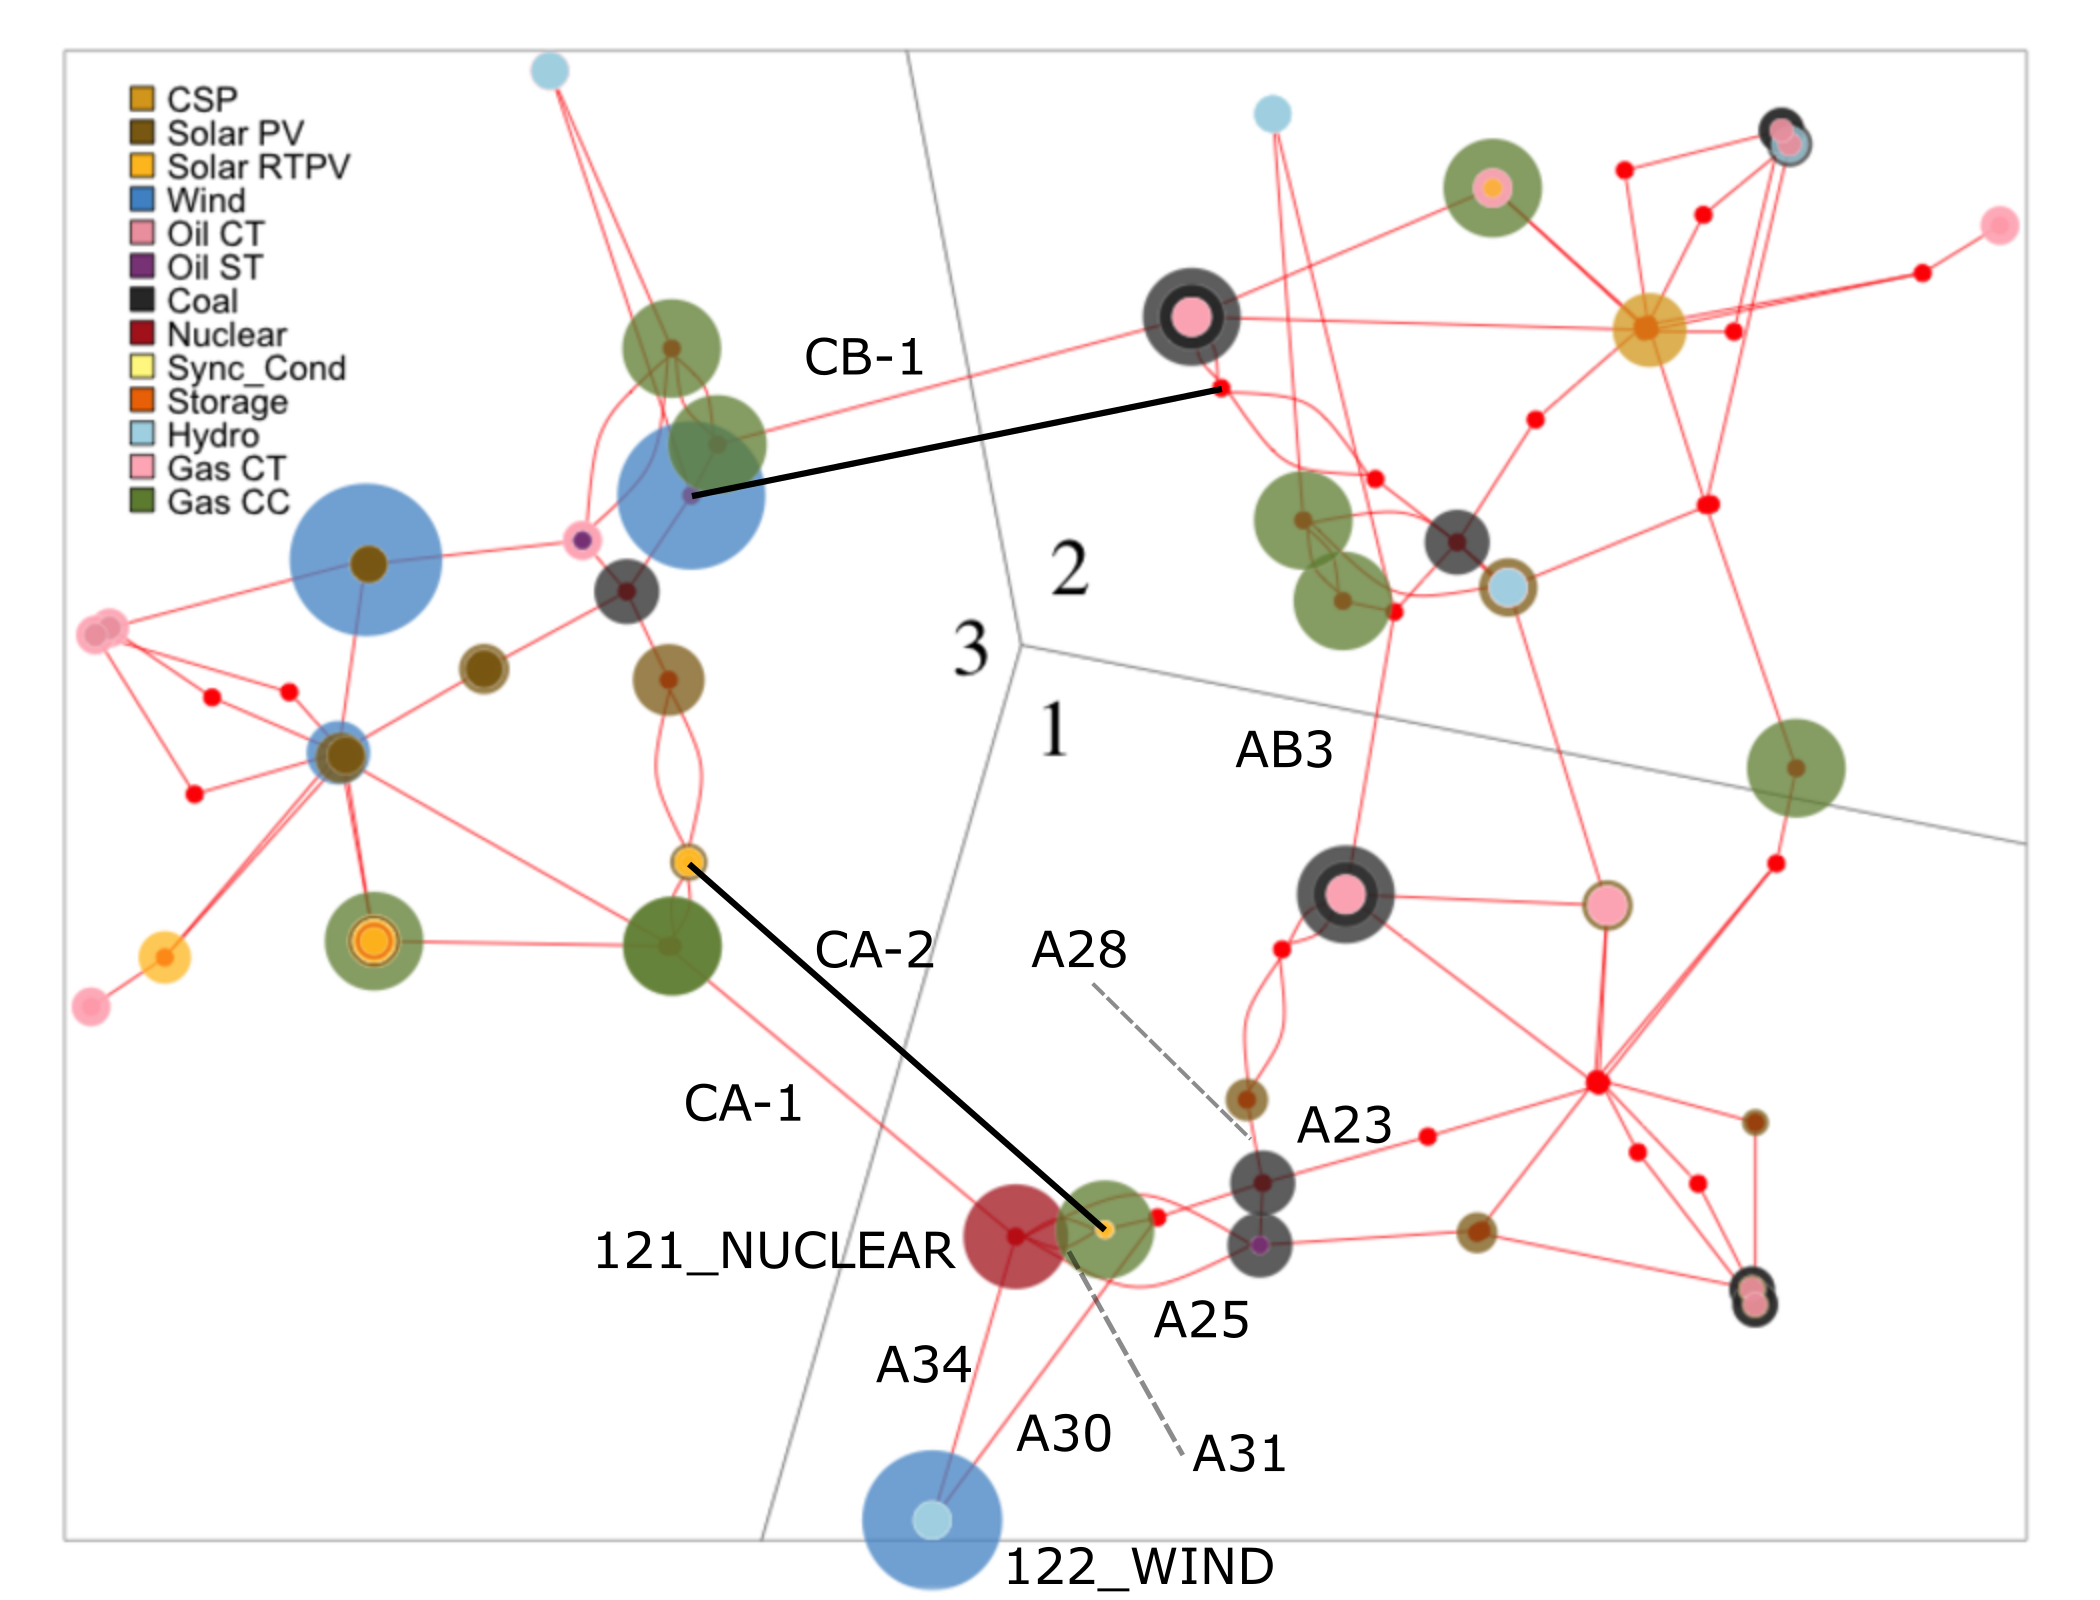
\includegraphics[width=0.8\linewidth]{Figs/RTS.png}
    \caption{Network layout of the RTS-GMLC from~\cite{RTS-GMLC}. New interconnections are represented in black.}
    \label{fig:RTS}
\end{figure}

For this work, two interconnections have been added to limit curtailment of the (very) large wind plants in zone 3 as shown in Figure~\ref{fig:RTS}. Other minor modifications have been done and are listed on \url{https://github.com/FredericSabot/PDSA-RTS-GMLC/tree/master/RTS-Data}. Hourly dispatches for typical days in January and July are shown in Figure~\ref{fig:dispatch}. The market model used is a locational marginal pricing (LMP) market model developed in~\cite{Prescient}. Figure~\ref{fig:dispatch} shows that high wind penetration (above 60\%) are sometimes reached especially for winter months during which load is relatively low. The RTS-GMLC data only includes a one-year time series realisation of renewable capacity factors and hydro inflows. Also, for the sake of simplicity, all assets (generation and transmission) are assumed to be always available. Therefore, only one MC year is considered.

\begin{figure}
\centering
\begin{tikzpicture}
\pgfplotsset{
/pgfplots/area cycle list/.style={/pgfplots/cycle list={%
{RedViolet,fill=red!75!black,mark=none},%
{black,fill=black,mark=none},%
{SeaGreen!40!white,fill=SeaGreen!40!white,mark=none},%
{LimeGreen!80!black,fill=LimeGreen!80!black,mark=none},%
% {pink,fill=pink,mark=none},%
{Cerulean,fill=Cerulean,mark=none},%
{Dandelion,fill=Dandelion,mark=none},%
}
},
}
\begin{groupplot}[
    group style={%
        columns=2,
        group name=plots,
        xlabels at=edge bottom,
        y descriptions at=edge left,
        horizontal sep =15pt,
    },
    xlabel = {Time [h]},
    ylabel = {Power [MW]},
    stack plots=y,%
    area style,
    xmin=0, xmax=24,
    xtick={0,8,16,24},
    ymin = 0, ymax=7500,
    tickpos=left,
    % ytick align=outside,
    % xtick align=outside,
    width=0.4\linewidth,
    height=0.4\linewidth,
]
\nextgroupplot
\addplot table [x=hour,y=nuclear] {Figs/dispatch_january.txt}
\closedcycle;
\addplot table [x=hour,y=coal] {Figs/dispatch_january.txt}
\closedcycle;
\addplot table [x=hour,y=hydro] {Figs/dispatch_january.txt}
\closedcycle;
\addplot table [x=hour,y=gas] {Figs/dispatch_january.txt}
\closedcycle;
% \addplot table [x=hour,y=oil] {Figs/dispatch_january.txt}
% \closedcycle;
\addplot table [x=hour,y=wind] {Figs/dispatch_january.txt}
\closedcycle;
\addplot table [x=hour,y=solar] {Figs/dispatch_january.txt}
\closedcycle;

\nextgroupplot[legend to name={DispatchLegend2},legend style={legend columns=6}]
\addplot table [x=hour,y=nuclear] {Figs/dispatch_july.txt}
\closedcycle;
\addplot table [x=hour,y=coal] {Figs/dispatch_july.txt}
\closedcycle;
\addplot table [x=hour,y=hydro] {Figs/dispatch_july.txt}
\closedcycle;
\addplot table [x=hour,y=gas] {Figs/dispatch_july.txt}
\closedcycle;
% \addplot table [x=hour,y=oil] {Figs/dispatch_july.txt}
% \closedcycle;
\addplot table [x=hour,y=wind] {Figs/dispatch_july.txt}
\closedcycle;
\addplot table [x=hour,y=solar] {Figs/dispatch_july.txt}
\closedcycle;

\legend{Nuclear, Coal, Hydro, Gas, Wind, Solar}

\end{groupplot}

\node[below] at (current bounding box.south)
      {\pgfplotslegendfromname{DispatchLegend2}};

\end{tikzpicture}
\caption{Market dispatch for a typical day in January (left) and July (right)}
\label{fig:dispatch}
\end{figure}

As there was no dynamic data in the original RTS-GMLC, they have been added in this thesis. Synchronous generators are represented with standard eighth order model and equipped with an IEEET1 exciter and a BPA GG (also known as WSCC type G) governor model as in~\cite{IEEE39Dynamic}. A different model is however used for hydro units as they have a fundamentally different behaviour than other types of units. The model used is an GOVHYDRO1 model. The machine, exciter and governor parameters are taken from annex D of~\cite{vittalBook}. This annex contains typical data for different types of machines (hydro, nuclear, coal, gas) and a wide range of rated powers (5~MW to 1.3~GW). So, for each generator of the test systems, parameters were taken from a machine in~\cite{vittalBook} that has the same type and that has the closest rated power. For hydro units, those parameters are completed with the ones in~\cite{hydroGov}. For inverter-based generation, the models from~\cite{ChaspierreThesis} are used. The protection system models (and associated uncertainty) are the same as in section~\ref{sec:protection_test_case} except load blinders have been added to distance protections. The blinders are set to avoid tripping for apparent impedances that correspond to a load of 150\% of the rated line current at 0.85~pu voltage and with a power factor angle of less than 30° following NERC recommendations~\cite{NERC_load_blinders}.

The contingencies considered in this example are three-phase faults occurring at one of the two extremities of lines. These faults are normally cleared by opening the faulted line in 100ms (N-1 contingency). However, it is also considered that there is a 0.1 probability that the primary protection fails and that the fault is thus cleared in 200ms (N-1 contingency with delayed clearing). Also, I consider a 0.01 probability that one breaker fails to open when clearing the fault. Breaker failure protection~\cite{HorowitzBook} is assumed to be installed in all substations and that they are able to clear the fault by opening a single adjacent line in 200ms (leading to an N-2 contingency). It has been checked that the system is always secure for N-1 contingencies with normal clearing time, these have thus not been considered in the PDSA. The contingencies listed above are line faults which are not cleared by the primary protection system due to protection failure or ``missed trips''. Another important class of protection failures are ``unwanted trips'', \ie trips that are not necessary to clear the fault and that thus unnecessarily disconnect elements. However, those are significantly more difficult to model as discussed in chapter~\ref{ch:protections} and are thus left for future work.

Only faults at the highest voltage level are considered which leads to a contingency list of 114 N-1 contingencies with delayed clearing and 594 N-2 contingencies. The frequency of line faults is taken as 2.5 faults per 100~km of line per year~\cite{FaultStatisticsFrance}\footnote{Due to lack of data, line fault probability is assumed independent of weather conditions. Fault and protection failure statistics significantly vary from country to country due to different weather and reliability and reporting practices (\eg \cite{GridPSA} reports a 0.27 fault per year and per 100~km of 400~kV overhead lines for the Finnish grid, while \cite{FaultStatisticsFrance} reports 2.5 in France). Data collection plans (as initiated by ENTSO-E~\cite{ENTSOE-PSA}) and failure mode and effect analysis (as demonstrated in~\cite{GridPSA}) should thus be performed to be able to fully trust the results of a PDSA.}.

The simulation of a given scenario provides with an estimate of the consequences of a contingency in terms of MW of load shed. This value can be translated into societal costs using the simple method described in section~\ref{sec:blackout_cost}. For the RTS and at average load (4350~MW), the cost of a complete blackout is thus estimated at 500M€. This is the value used for \(M_C\). Dynamic simulations are performed using \Dynawo{}~\cite{Dynawo} on 10 32-cores AMD EPYC Rome 7542 CPU's at 2.9 GHz.

Due to lack of time, loads where represented using a constant impedance load model in parallel with a simple motor model accounting for 30\% of the load. For grids with high shares of distributed energy sources, loads should instead be modelled using dynamic equivalents as discussed in chapter~\ref{ch:distrib}. The method proposed in chapter~\ref{ch:distrib} requires to simulate each scenario twice: once with 5-equivalents and once with 95-equivalents which double computation time. To limit this computation time, only the 95-equivalent could be used as it usually lead to more conservative results (especially for secure scenarios).

As for the other test cases in this thesis, the grid used in this example only has models for short-term stability as it is the focus of this thesis. However, while purely-fast cascades are becoming more common, there are still many cascades that start as slow cascades and latter transition to fast cascades if they cannot be stopped in the slow phase. To model these cascades that develop on a large range of timescales, it would be convenient to use simulators that can simulate such large ranges of timescales thanks to a variable integration time step such as Eurostag~\cite{STAG} or \Dynawo{}~\cite{Dynawo}. Alternatively, the slow and fast phases could be simulated separately as proposed in~\cite{TwoLevelPSA}. The advantage of this second approach is that more MC samples can be simulated during the slow phase (that is less computationally expensive to simulate). However, it requires predicting when a given cascade transition from the slow to the fast phase.



\section{Application of the proposed PDSA methodology}
\label{sec:PDSA_results}

This section describes the application of the proposed PDSA methodology to the RTS-GMLC with a focus on aspects related to sampling and computation time. The ``physical'' results will be described in section~\ref{sec:PDSA_interpretation} along with the discussion on how to use these results to enhance the security of the system.

% This section is organised similarly to the methodology section with section~\ref{sec:PDSA_results_sampling} discussing the sampling process and computational burden of the PDSA, section~\ref{sec:PDSA_results_screening} discussing the performance of the screening process and its impact on accuracy and computation time, section~\ref{sec:PDSA_results_protections} analysing the impact of protection-related uncertainties on fast cascading outages,


\subsection{Sampling of operating conditions}
\label{sec:PDSA_results_sampling}

A first PDSA has been performed without screening of scenarios to be used as a reference. An \(\epsilon\) of 1\% has been used in this example for the stopping criterion~(\ref{eq:stop}). The main results of this analysis are given in Table~\ref{tab:summary-N1N2}. It shows that N-1 contingencies with delayed clearing and N-2 contingencies have a similar contribution to the total risk. Also, while there are more N-2 contingencies than N-1 contingencies (594 vs 114), N-2 contingencies require fewer simulations, and therefore less computation time than N-1 contingencies. In total, 152,138 scenarios are considered, leading to 157,346 simulations (to account for protection-related uncertainties). 4329 scenarios are found to be unsecure, and 7 lead to convergence issues in the time-domain simulation. This relatively small number of unsecure scenarios indicates that screening of scenarios could significantly reduce computation time.

\begin{table}
\centering
\caption{Contribution to total risk and computation time of delayed clearing N-1 contingencies and N-2 contingencies (without screening)}
\label{tab:summary-N1N2}
\begin{tabular}{@{}lll@{}}
\toprule
                                 & N-1 with delayed clearing  & N-2 \\ \midrule
Risk (M€/y) & 8.6 & 12.4 \\
Number of simulations            & 97,503 & 59,648 \\
Computation time (core-h)        & 1046  & 656 \\
Average computation time per simulation (s) & 38.6 & 39.6 \\ \bottomrule
\end{tabular}
\end{table}


This is because N-1 contingencies (with delayed clearing) are contingencies that are more frequent than N-2 contingencies but infrequently lead to significant consequences. It is thus necessary to sample many operating conditions to obtain a statistically accurate risk and guarantee a sufficient coverage of the likely operating conditions.

Figure~\ref{fig:indic_N1} (resp. Figure~\ref{fig:indic_N2}) shows the number of simulations performed for all N-1 (resp. N-2) contingencies and the associated standard error (decomposed in terms of variance and coverage). It shows that for most contingencies the coverage part of the SE is dominant compared to the variance part. For these contingencies, the SE bound reduces to

\begin{equation}
  SE_i \lesssim \frac{f_i}{N_i} \sqrt{3 \beta_i^2}
\end{equation}

\noindent and the number of simulations needed to satisfy the stopping criterion (\ref{eq:stop}) is thus directly proportional to the frequency of the contingency. For contingencies with non-negligible variance, the number of simulations needed is higher which explains the spikes of \(N_i\) in Figure~\ref{fig:indic_N1} and Figure~\ref{fig:indic_N2}.


\begin{figure}
\centering
\begin{tikzpicture}
\pgfplotsset{width=0.8\linewidth}
\begin{groupplot}[
    group style={
        group name=my plots,
        group size=1 by 2,
        xlabels at=edge bottom,
        xticklabels at=edge bottom,
        vertical sep=20pt,
    },
    width=0.8\linewidth,
    height=5cm,
    xlabel=Contingency ID,
    xmin=1, xmax=114,
    ymin=0,
    yticklabel style={/pgf/number format/fixed},
    tickpos=left,
    ytick align=outside,
    xtick align=outside,
]
\nextgroupplot[ylabel=\(N_i\), height=4cm]
\addplot+ [mark=none] table [x=id,y=N_static] {Figs/N_N1.txt};

\nextgroupplot[
    ylabel style={align=center}, ylabel=Statistical accuracy\\{[M€/y]},
    legend style={legend columns=2}, ymax=0.34]

\addplot+ [ybar interval, fill, mark=none] table [x=id,y expr=\thisrow{indic_1}*1.609344] {Figs/N_N1.txt};  % TODO: remove mi to km conversion if computations are rerun
\addplot+ [mark=none] table [x=id,y expr=\thisrow{indic_2}*1.609344] {Figs/N_N1.txt};
\addlegendentry{Variance}
\addlegendentry{Coverage}
\end{groupplot}
\end{tikzpicture}
\caption{Number of sampled operating conditions and statistical accuracy for all delayed-clearing N-1 contingencies sorted in decreasing order of likelihood}
\label{fig:indic_N1}
% \end{figure}
\vspace{0.7cm}
% \begin{figure}
\centering
\begin{tikzpicture}
\pgfplotsset{width=0.8\linewidth}
\begin{groupplot}[
    group style={
        group name=my plots,
        group size=1 by 2,
        xlabels at=edge bottom,
        xticklabels at=edge bottom,
        vertical sep=20pt,
    },
    width=0.8\linewidth,
    height=5cm,
    xlabel=Contingency ID,
    xmin=1, xmax=594,
    ymin=0,
    yticklabel style={/pgf/number format/fixed},
    tickpos=left,
    ytick align=outside,
    xtick align=outside,
]
\nextgroupplot[ylabel=\(N_i\), height=4cm]
\addplot+ [mark=none] table [x=id,y=N_static] {Figs/N_N2.txt};

\nextgroupplot[
  ylabel style={align=center}, ylabel=Statistical accuracy\\{[M€/y]},
  legend style={legend columns=2}, ymax=0.34]

  \addplot+ [ybar interval, fill, mark=none] table [x=id,y expr=\thisrow{indic_1}*1.609344] {Figs/N_N2.txt};
  \addplot+ [mark=none] table [x=id,y expr=\thisrow{indic_2}*1.609344] {Figs/N_N2.txt};
\addlegendentry{Variance}
\addlegendentry{Coverage}
\end{groupplot}
\end{tikzpicture}
\caption{Number of sampled operating conditions and statistical accuracy for all N-2 contingencies sorted in decreasing order of likelihood}
\label{fig:indic_N2}
\end{figure}


It is interesting to see that when aiming to minimise the SE of the risk contribution of \emph{individual} contingencies, the best strategy is basically to use a crude MC approach (\ie sampling contingencies proportionally to their frequency of occurrence) (except for a few contingencies with high variance). In a crude MC approach, the total risk can be estimated as

\begin{equation}
  R = \left(\sum_i f_i\right) \left(\frac{1}{N} \sum_s c_s\right)
\end{equation}

\noindent where \(c_s\) are the consequences of the \(s\)th sample (random contingency and initial state). Using the same development as to derive equation~\ref{eq:SE_bound}, the following bound can be obtained for the SE of the total risk.

\begin{equation}
  \label{eq:SE_total}
  SE \leq \left(\sum_i f_i\right) \sqrt{\frac{\tilde{\sigma}^2}{N} + \frac{3 \beta^2}{N^2}}
\end{equation}

\noindent where \(\tilde{\sigma}\), \(\beta\), and \(N\) have the same definitions as \(\tilde{\sigma_i}\), \(\beta_i\), and \(N_i\) but for the total risk instead of individual contingencies. Figure~\ref{fig:SE_total} shows how this SE evolves with the number of samples. After 150,000 samples (roughly the number of simulations performed in this study, cf. Table~\ref{tab:summary-N1N2}), the coverage term of SE is 4.3 smaller than the variance term while it was strongly dominant for the SE of individual contingencies. This is because the coverage term accounts for the likelihood of having missed unsecure regions during sampling, and while this likelihood is relatively high for individual contingencies, it is unlikely to miss unsecure regions for all of them. Figure~\ref{fig:SE_total} shows the coverage term becomes smaller than the variance term after roughly 8000 samples. Thus, if one is only interested in the total risk and not in the risk of individual contingencies (for some reason), then variance-reduction techniques become viable after this point.

\begin{figure}
\centering
\begin{tikzpicture}
\pgfplotsset{width=0.6\linewidth}
\begin{axis}[
    xlabel={Number of samples},
    xmin=1000, xmax=150000,
    ymin=0, ymax=8,
    xmode=log,
    grid,
    log ticks with fixed point,
    ylabel= {SE [M€/y]},
    legend cell align=left,
    legend style={at={(1,1)},anchor=north east},
    ]

    \addplot+ [mark=none, dashed] table [x=x,y expr=\thisrow{sigma}*1.609344] {Figs/total_risk_SE.txt};
    \addplot+ [mark=none, dashdotted] table [x=x,y expr=\thisrow{coverage}*1.609344] {Figs/total_risk_SE.txt};
    \addplot+ [mark=none] table [x=x,y expr=\thisrow{SE}*1.609344] {Figs/total_risk_SE.txt};
    \addplot+ [mark=none, gray, dashed, domain=500:150000, samples=2] {0.05 * 13.226341374847571 * 1.609344};

    \addlegendentry{Variance}
    \addlegendentry{Coverage}
    \addlegendentry{Total SE}
    \addlegendentry{5\% of total risk}

\end{axis}
\end{tikzpicture}
\caption{Evolution of the SE of the total risk with the number of samples}
\label{fig:SE_total}
\end{figure}

\begin{figure}
  \centering
  \begin{tikzpicture}
  \pgfplotsset{width=0.8\linewidth}
  \begin{axis}[
      height=5cm,
      xlabel=Contingency ID,
      xmin=0.5, xmax=20.5,
      ymin=0,
      yticklabel style={/pgf/number format/fixed},
      ylabel=Risk {[M€/y]},
      xtick={1,2,...,20},
  ]

  \addplot+ [ybar, ybar legend, fill, mark=none, bar width=5pt] table [x=id,y expr=\thisrow{cost}*1.609344] {Figs/critical_SE.txt};
  \addplot+ [mark=none, domain=0:21] {0.01 * 13.226341374847571 * 1.609344};

  \addlegendentry{Risk}
  \addlegendentry{\(SE_i\)}

  \end{axis}
  \end{tikzpicture}
  \caption{Risk of the 20 most critical contingencies and associated SE}
  \label{fig:SE_individual}
\end{figure}

It can be noted that, for a given number of samples, the statistical accuracy of the total risk estimate is better than the one of the individual contingencies. Indeed, Figure~\ref{fig:SE_total} shows that with 150,000 samples, the SE of the total risk is smaller than 5\%. On the other hand, Figure~\ref{fig:SE_individual} shows a SE higher than 50\% for all contingencies except the 10 most critical ones.


\subsection{Sampling of protection-related uncertainties}
\label{sec:PDSA_results_protections}

The results discussed above have been obtained by running 5 MC simulations for each scenario for which protection-related uncertainties are expected to have an impact. This was the case for a fifth (834 out of 4329) of unsecure scenarios. Of these, half (408 out of 834) led to different consequences depending on the sampled protection system parameters. In the remaining half, the cascading path was affected by protection-related uncertainties, but the final consequences were not. As discussed in section~\ref{sec:protection_results}, there are two main reasons for this. The first is that changing the order of protection operations does not always impact the general evolution of the cascade. The second is that the operation of an additional protection system does not necessarily impact the consequences, for example, if it occurs in an island of the system that will nevertheless collapse.

Performing 5 MC simulations for each scenario impacted by protection-related uncertainties can be viewed as a way to perform importance sampling. However, as shown above, a crude MC approach is more efficient for most contingencies. Theoretically, it would thus be more efficient to draw one sample of protection-related parameters for each sample of operating conditions. But in practice, the proposed approach gives more intuitive results because it allows one to separate the impact of operating conditions and of protection parameters.

Also, it can be argued that using an indicator to predict which scenarios are sensitive to protection-related uncertainties increases coverage as one sample directly accounts for all possible values of protection parameters, reducing the dimension of the uncertainty space and the likelihood of missing critical regions. In any case, the impact on computation time is relatively limited as the scenarios that are secure and not affected by protection-related uncertainties take most of the computation time.


% Comparing MC algorithms is often performed using a Figure of Merit (FoM)
%
% \begin{equation}
% FoM_i = \frac{1}{\tilde{\sigma_i}^2 N^T_i}
% \end{equation}
%
% where \(R_i\) is the risk associated to contingency \(i\), and \(N^T_i\) is the total number of simulations performed for contingency \(i\). Fig.~\ref{fig:FoM} shows that the PDSA performed without the indicator has a higher FoM and is thus more efficient for most of the contingencies. Despite the above, we still recommend the use of the indicator as (i) it helps in the interpretation of the simulation results by decoupling the impact of static and protection-related uncertainties, and (ii) it acts as a form of robustness analysis (for protection-related uncertainties only), at the cost of a small increase in computation time.
%
% \begin{figure}  % FoM figure should be updated (sigma should be lower with indicator). Anyway, this neglects coverage, so not super useful
% \centering
% \begin{tikzpicture}
% \pgfplotsset{width=0.8\linewidth}
% \begin{groupplot}[
%     group style={
%         group name=my plots,
%         group size=1 by 3,
%         xlabels at=edge bottom,
%         xticklabels at=edge bottom,
%         vertical sep=20pt
%     },
%     height=4cm,
%     xlabel=Contingency ID,
%     xmin=1, xmax=10,
%     ymin=0,
%     tickpos=left,
%     ytick align=outside,
%     xtick align=outside,
% ]
% \nextgroupplot[ylabel=\(S_i\) {[\%]}, ymax=50]
% \addplot+ [mark=none] table [x=id,y=share] {Figs/FoM.txt};
% \nextgroupplot[
%     ylabel=\(\sigma_i\),
%     legend cell align=left,
%     legend style={at={(1,1)},anchor=north east}]
% \addplot+ [mark=none] table [x=id,y=std_dev] {Figs/FoM.txt};
% \addplot+ [mark=none] table [x=id,y=std_dev_no_indic] {Figs/FoM.txt};
% \nextgroupplot[
%     ylabel=\(FoM_i\),
%     legend to name={CommonLegend},legend style={legend columns=2}]
% \addplot+ [mark=none] table [x=id,y=FoM] {Figs/FoM.txt};
% \addplot+ [mark=none] table [x=id,y=FoM_no_indic] {Figs/FoM.txt};
% \addlegendentry{With indicator}
% \addlegendentry{Without indicator}
% \end{groupplot}
% \node[below] at (current bounding box.south)
%       {\pgfplotslegendfromname{CommonLegend}};
% \end{tikzpicture}
% \caption{Share of operating conditions \(S_i\) for which protection-related uncertainties have an impact, standard deviation \(\sigma_i\), and figure of merit \(FoM_i\) of the 10 N-2 contingencies with the largest \(S_i\)}
% \label{fig:FoM}
% \end{figure}


\subsection{Missing trips during cascades}
\label{sec:PDSA_results_missing_trips}

Some works (\eg~\cite{Faghihi, DCATphase1}) consider that there might be ``missing trips'' during the evolution of the cascade. Indeed, each time a protection system operates during a cascade, there is also some probability that it fails to operate. This can be considered by splitting the simulation in two branches when one protection operates: one where the protection actually operates and one where it fails to; each associated with some probability.

Due to time constraints, this has not been considered in this thesis. However, an estimation of the risk associated with those missing trips can be done based on the results of the present analysis. Indeed, for each simulation performed, the associated sequence of tripping events is saved to allow for further analysis. The frequency of protection system operations (not accounting for fault clearing) can thus be estimated at 0.35 per year. This can be compared to the 17.9 contingencies per year of the RTS (11.7 for delayed-clearing N-1 contingencies and 6.2 for N-2 contingencies). This figure does not account for under-frequency load shedding (UFLS) relay trips because the failure of a single UFLS relay is unlikely to affect the evolution of a cascade. Generator protections are also not included in this figure as missing trips of generators are made very unlikely due to the high consequences for the generator if it is not disconnected when needed.

Based on this figure, assuming a probability of protection failure to operate of 0.01, and assuming that any protection system failure to operate during a cascade leads to a full blackout leads to a risk of 2.83~M€/y. This risk is thus negligible compared to the 28.8~M€/y risk computed without considering the possible failure of protection to operate during cascades. Moreover, this 2.83~M€/y figure is very conservative as it assumes all protection failures to operate lead to a full blackout. Actually, since most protection systems aim to protect individual elements and not the grid itself, a failure to operate during a cascade will not necessarily have a negative impact on the cascade propagation. The failure of system integrity protection schemes could be considered. However, they are often designed to have a very high level of reliability, so it would make more sense in a possibilistic approach rather than a probabilistic one.

This section has discussed the risk associated with missing trips, but, as discussed previously, unwanted trips (both directly following fault clearing and during the cascade propagation) should be studied in further work.


\subsection{Screening}
\label{sec:PDSA_results_screening}

We now study how the addition of a screening process impacts the accuracy and computational burden of the PDSA. The main results are given in Table~\ref{tab:screening}. First, it is important to notice that even though the contingencies considered in this analysis are relatively severe (compared to the N-1 contingencies with normal clearing time the system has been designed to withstand), only 3\% of the sampled scenarios (4329 out of around 152,138) lead to consequences (around 2\% for delayed-clearing N-1 scenarios, and 4\% for N-2 scenarios). Therefore, without screening, 95\% of the computation time is wasted on secure scenarios (not 97\%, as an unsecure scenario takes on average more time to simulate than a secure one).

With perfect screening, the computational burden of the PDSA can thus be reduced by a factor 20. The screening process used in this work does not reach this performance however. It has a low false negative (FN) rate, \ie very few unsecure scenarios are missed, so it has a low impact on the PDSA accuracy (only 4\% of the total risk is missed). However, it has a high false positive (FP) rate, \ie many secure scenarios are flagged as unsecure and therefore unnecessarily simulated. Screening thus only speeds up the PDSA by a factor 1.94, way less than the theoretical limit of 20.

\begin{table}
  \centering
  \caption{Performance of the screening process and impact on the PDSA accuracy and computation time}
  \label{tab:screening}
  \begin{tabular}{@{}lllllll@{}}
    \toprule
    \multirow{2}{*}{Contingencies} &
      \multicolumn{2}{l}{Unsecure cases} &
      \multicolumn{2}{l}{Secure cases} &
      \multirow{2}{*}{\begin{tabular}[c]{@{}l@{}}Missed\\ risk (\%)\end{tabular}} &
      \multirow{2}{*}{Speed-up} \\ \cmidrule(lr){2-3} \cmidrule(lr){4-5}
        & FN & TP   & FP     & TN     &     &      \\ \midrule
    N-1 with delayed clearing & 4  & 1553 & 40,100 & 52,400 & 0.3 & 2.01 \\
    N-2 & 81 & 1847 & 22,300 & 25,200 & 6.4 & 1.81 \\
    All & 85 & 3400 & 62,400 & 77,800 & 4.0 & 1.94 \\ \bottomrule
  \end{tabular}
\end{table}

This is mainly because the EEA underestimate CCT in this case due to the large penetration of inverter-based generators. Indeed, due to their low capacity factors, inverter-based generators often have room to provide fast voltage support which helps with the angular stability of synchronous generators. Table~\ref{tab:CCT_margin} shows that when using a CCT margin of -20ms in the screening process, \ie assuming that faults cleared in 200ms are secure if the EEA predicts a CCT larger than 180ms, a speed-up of 3.5 can be obtained but at the cost of missing 16.6\% of the total risk. Better stability indicators should be developed if higher speed-ups and/or lower impact on accuracy are desired.

\begin{table}
  \centering
  \caption{Impact of the CCT margin on screening performance}
  \label{tab:CCT_margin}
  \begin{tabular}{@{}lll@{}}
  \toprule
  CCT margin (ms) & Missed risk (\%) & Speed-up \\ \midrule
  50  & 4.0  & 1.94 \\
  0   & 9.3  & 2.75 \\
  -20 & 16.6 & 3.49 \\ \bottomrule
  \end{tabular}
\end{table}

It should be noted that the screening does not affect the risk estimate of all contingencies in the same way. In the case of the negative 20ms CCT margin, the risk estimates for the first 10 most critical contingencies are not affected by the screening process, except for the 2nd most critical contingency that is almost entirely missed and the 4th whose risk is underestimated by 25\%. With 0 margin, the risk of the 2nd most critical contingency is underestimated by 35\% which is more acceptable. With a positive 50ms margin, none of the first 10 most critical contingencies are underestimated by the screening process.

% 0.18 CCT threshold
% Rank 2, A25-1_end1-BREAKER_end1-A25-2, misses: 55/82, max shedding: 100.0
% Rank 4, A23_end2-BREAKER_end2-A28, misses: 6/22, max shedding: 100.0
% Rank 6, C22_end1_DELAYED, misses: 1/146, max shedding: 10.0
% Rank 11, A23_end1-BREAKER_end2-A28, misses: 7/7, max shedding: 100.0
% Rank 12, A27_end2-BREAKER_end1-A24, misses: 4/5, max shedding: 100.0
% Rank 14, CA-2_end2_DELAYED, misses: 1/9, max shedding: 67.84
% Rank 17, B21_end2_DELAYED, misses: 2/73, max shedding: 3.495
% Rank 18, A27_end1-BREAKER_end1-A24, misses: 2/5, max shedding: 100.0

% 0.2
% Rank 2, A25-1_end1-BREAKER_end1-A25-2, misses: 30/82, max shedding: 100.0
% Rank 4, A23_end2-BREAKER_end2-A28, misses: 1/22, max shedding: 100.0
% Rank 6, C22_end1_DELAYED, misses: 1/146, max shedding: 10.0
% Rank 11, A23_end1-BREAKER_end2-A28, misses: 7/7, max shedding: 100.0
% Rank 12, A27_end2-BREAKER_end1-A24, misses: 1/5, max shedding: 100.0
% Rank 18, A27_end1-BREAKER_end1-A24, misses: 1/5, max shedding: 100.0

% 0.25
% Rank 11, A23_end1-BREAKER_end2-A28, misses: 7/7, max shedding: 100.0
% Rank 22, A28_end2-BREAKER_end1-A23, misses: 4/6, max shedding: 100.0

\section{Interpreting the results and enhancing security}
\label{sec:PDSA_interpretation}

Once all necessary simulations have been performed, the results of the PDSA can be analysed. A first intuitive interpretation of the results is proposed in section~\ref{sec:PDSA_results_intuitive}. However, as the PDSA produces thousands of unsecure scenarios (and even more secure ones), it is not possible to review each scenario in details. To alleviate this issue, machine learning techniques can be used. Basic machine learning techniques are thus used in section~\ref{sec:PDSA_ML} to help with the interpretation of the results and to enhance the security of the system.

\subsection{Intuitive interpretation of the results}
\label{sec:PDSA_results_intuitive}

Table~\ref{tab:critical_contingencies} shows a summary of the PDSA results for the 10 most critical contingencies. It should be noted that these 10 contingencies (out of 708) contribute for 44\% of the total risk. This shows that significant reduction of the risk could potentially be obtained by targetting those specific contingencies. Moreover, most of these contingencies concern lines that are in the same region (in the South of Figure~\ref{fig:RTS-copy}) highlighting the potential to solve multiple issues in one go.

\afterpage{%
\clearpage% Flush earlier floats (otherwise order might not be correct)
% \thispagestyle{empty}% empty page style (actually fine with headers)
\begin{landscape}% Landscape page
\centering

\begin{figure}
\centering
\begin{minipage}{\linewidth}
\begin{minipage}[c]{0.58\linewidth}
  \strut\vspace*{-\baselineskip}\newline % Minipage vertical allignement black magic
  % \centering
  \captionof{table}{Results of the PDSA for the 10 most critical contingencies. Line locations are given in Figure~\ref{fig:RTS-copy}.}
  \vspace*{0.5\baselineskip}
  \begin{tabular}{@{}lllllll@{}}
    \toprule
    \multicolumn{2}{c}{Contingency} &
      \multirow{2}{*}{\begin{tabular}[c]{@{}l@{}}Risk\\ {[}M€/y{]}\end{tabular}} &
      \multirow{2}{*}{\begin{tabular}[c]{@{}l@{}}Frequency\\ {[}/y{]}\end{tabular}} &
      \multirow{2}{*}{\begin{tabular}[c]{@{}l@{}}Share of unsecure\\ operating points {[}\%{]}\end{tabular}} &
      \multicolumn{2}{c}{Load shed {[}\%{]}} \\ \cmidrule(r){1-2} \cmidrule(l){6-7}
    Fault  & Adj. line &        &         &      & Mean\(^a\) & Max  \\ \midrule
    A34    & /         & 2.22  & 0.12   & 20.3 & 28.0 & 100  \\
    A25-1  & A25-2     & 1.87  & 0.017  & 18.9 & 69.7 & 100  \\
    CA-1   & /         & 1.66  & 0.17   & 11.6 & 21.4 & 100  \\
    A23    & A28       & 0.72 & 0.0068  & 18.3 & 81.9 & 100  \\
    CB-1   & /         & 0.68 & 0.18    & 8.5  & 15.4 & 36.5 \\
    C22    & /         & 0.60 & 0.15    & 12.2 & 10.8 & 25   \\
    A34    & A25       & 0.56 & 0.012   & 38.0 & 30.3 & 100  \\
    AB3    & /         & 0.56 & 0.13    & 7.1  & 15.5 & 100  \\
    A25    & /         & 0.55 & 0.17    & 6.8  & 14.5 & 91.3 \\
    A34    & CA-1      & 0.51 & 0.012   & 32.7 & 33.4 & 94.5 \\
    Others & /         & 12.4 & 17.0    & /    & /    & 100  \\ \bottomrule
    \multicolumn{7}{l}{\(^a\) Mean load shedding accounts for unsecure operating points only} \\
    \end{tabular}
  \label{tab:critical_contingencies}
\end{minipage}
\hfill
\begin{minipage}[c]{0.42\linewidth}
  \strut\vspace*{-\baselineskip}\newline % Minipage vertical allignement black magic
  \centering
  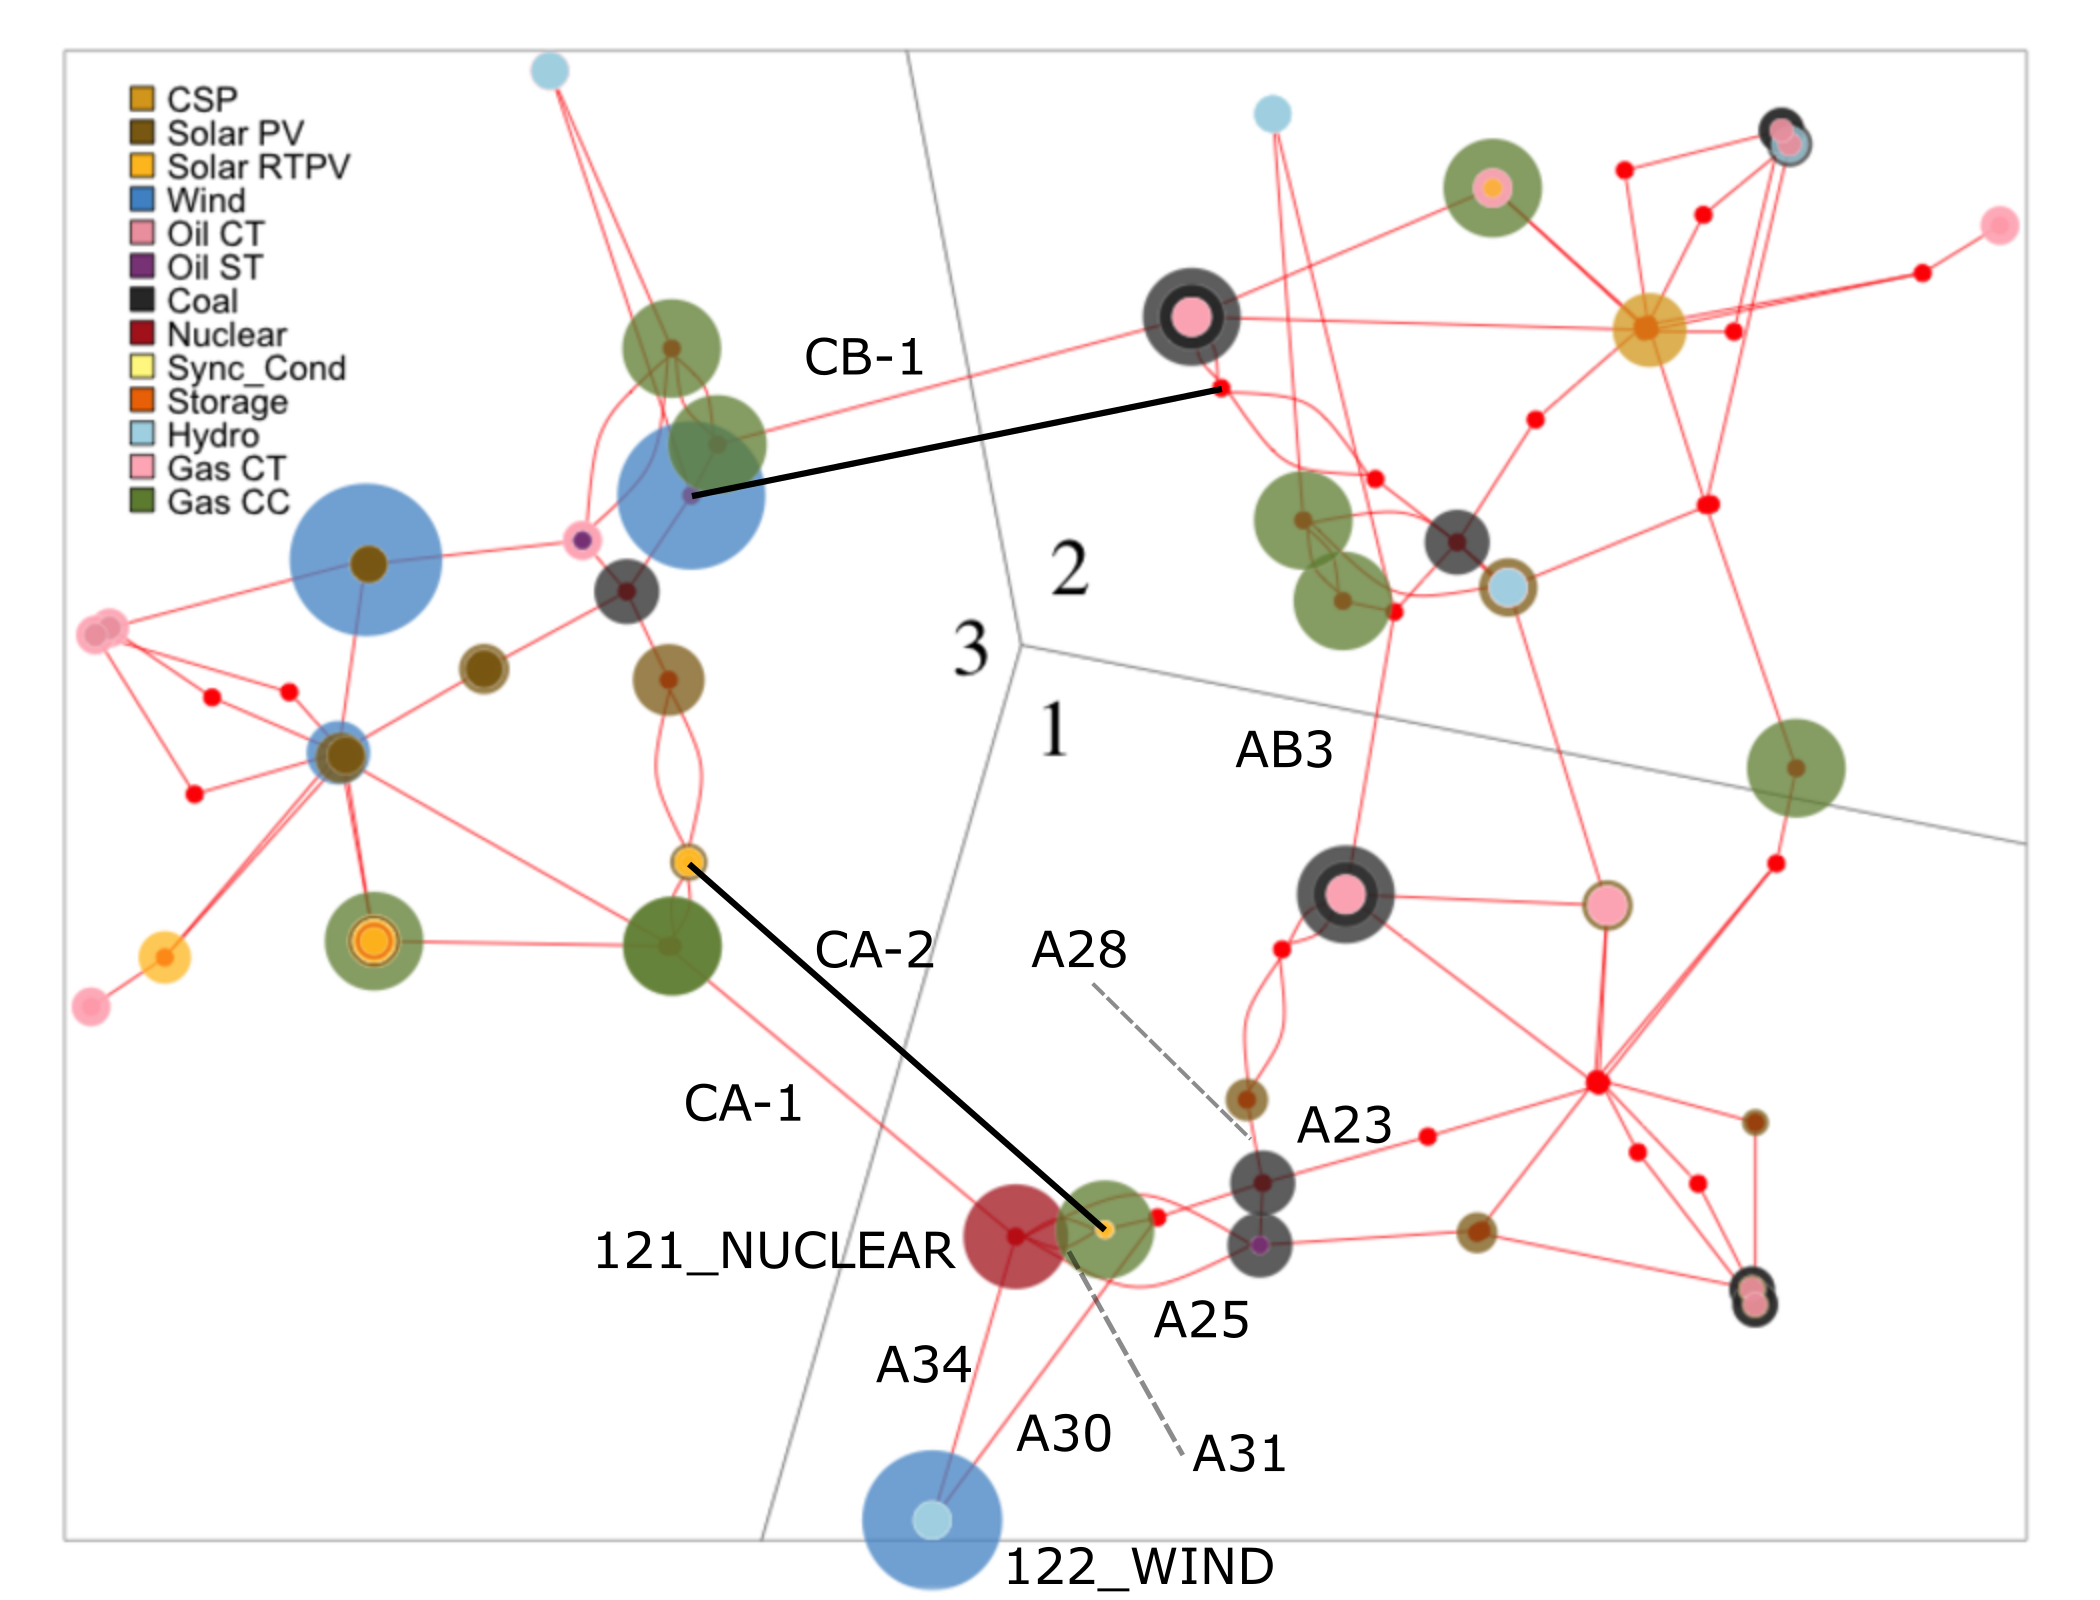
\includegraphics[width=0.8\linewidth]{Figs/RTS.png}
  \captionof{figure}{Network layout of the RTS-GMLC copied from Figure~\ref{fig:RTS} for convenience}
  \label{fig:RTS-copy}
\end{minipage}
\end{minipage}
\end{figure}


\begin{table}
\centering
\caption{Examples of samples for the most critical contingency (fault on line A34 with delayed clearing). Trips beyond the first three are not shown.}
\label{tab:samples_A34}
\begin{tabular}{@{}lllllll@{}}
  \toprule
  \begin{tabular}[c]{@{}l@{}}Hour\\ of year\end{tabular} & \begin{tabular}[c]{@{}l@{}}Load\\ shedding {[}\%{]}\end{tabular} & Trip 1 & Trip 2 & Trip 3 & \begin{tabular}[c]{@{}l@{}}Uncertain\\ protection impact\end{tabular} & \begin{tabular}[c]{@{}l@{}}Share of scenarios\\ with same initial 2 trips\end{tabular} \\ \midrule
  4633 & 0  & /                           & /                         & /                     & No            & 73.8 \\
  4103 & 51 & A30\_side2\_Distance\(^a\)  & 121\_NUCLEAR\_Angle\(^b\) & 122\_WIND\(^c\)       & Missing trips & 2.2  \\
  7634 & 40 & 121\_NUCLEAR\_Angle         & A30\_side2\_Distance      & 122\_WIND             & No            & 10.0 \\
  291  & 0  & 121\_NUCLEAR\_Angle         & /                         & /                     & No            & 5.3  \\
  8402 & 10 & 121\_NUCLEAR\_Angle         & UFLS\(^d\)                & /                     & No            & 3.9  \\
  8686 & 42 & A30\_side2\_Distance        & CA-1\_side1\_Distance     & 122\_WIND             & Missing trips & 0.6  \\
  1446 & 90 & CA-2\_side2\_Distance       & CA-1\_side2\_Distance     & A30\_side2\_Distance  & Missing trips & 0.8  \\ \bottomrule
  \multicolumn{6}{l}{\(^a\) Trip of line A30 by the distance protection on the second side of the line} \\
  \multicolumn{6}{l}{\(^b\) Trip of the nuclear power plant at bus 121 following loss of synchronism} \\
  \multicolumn{6}{l}{\(^c\) Trip of the wind farm at bus 122} \\
  \multicolumn{6}{l}{\(^d\) Under-frequency load shedding} \\
  \end{tabular}
\end{table}

% 73.8425925925926 ()
% 10.030864197530864 ('121_NUCLEAR_1_InternalAngle', 'A30_side2_Distance')
% 5.324074074074074 ('121_NUCLEAR_1_InternalAngle',)
% 3.8580246913580245 ('121_NUCLEAR_1_InternalAngle', 'UFLS')
% 2.2376543209876543 ('A30_side2_Distance', '121_NUCLEAR_1_InternalAngle')
% 0.7716049382716049 ('CA-2_side2_Distance', 'CA-1_side2_Distance')
% 0.6172839506172839 ('A30_side2_Distance', '122_WIND_1')

\end{landscape}
\clearpage% Flush page
}


However, Table~\ref{tab:critical_contingencies} does not explain why those contingencies are unsecure nor how to make them more secure. Table~\ref{tab:samples_A34} does a first step by showing a few samples (7 out of 1274) of the most critical contingency (fault on line A34 with delayed fault clearing). The table shows that the contingency can lead to different trip sequences depending on the operating conditions leading to different consequences. Actually, upon further analysis, all sequences are initiated due to the loss of synchronism of the nuclear power plant located in bus 121 (121\_NUCLEAR in Figure~\ref{fig:RTS-copy}).

Indeed, Figure~\ref{fig:A34_voltage} shows the voltage evolution for two of these cases (hours 7634 and 8402). In both cases, voltage at some buses stay depressed after fault clearing due to the loss of synchronism of the nuclear generator. Also, following the fault, line A34 is disconnected and the wind farm at bus 121 (121\_WIND) only remain connected to the rest of the system through line A30. And due to the depressed voltages, the wind farm is not able to push its power through this single line (that connects bus 121 to bus 117). In some cases (\eg Figure~\ref{fig:A34_voltage_7634}), this leads to trip of line A30 by distance protection. In other cases (\eg Figure~\ref{fig:A34_voltage_8402}), the distance protection of line A30 is armed, but the nuclear generator is disconnected, allowing for voltages to recover before the distance protection sends a trip signal.

These different possible sequences lead to different consequences. Indeed, in the former, both a nuclear power plant (of 400~MW) and a large wind farm (750~MW installed capacity, compared to the total load that varies between 3 and 7.5~GW) are disconnected leading to 30 to 50\% of load shedding (depending on operating conditions) by UFLS relays. In the latter, only the nuclear power plant is disconnected, so at most 15\% of the load has to be shed.

The two last cases in Table~\ref{tab:samples_A34} are also initiated by the loss of synchronism of the nuclear power plant at bus 121, however, they also lead to the disconnection of lines CA-1 and CA-2 that connect regions 1 and 3 together (by distance protection due to high flows from region 1 to region 3). These cases thus lead to more complex cascades with higher amounts of load shedding.

It should be noted that, for the contingency of line A34 with delayed clearing, 1253 out of 1296 sampled scenarios lead to the same first two initial trips as the scenarios listed in Table~\ref{tab:samples_A34}. By grouping scenarios that have the same starting tripping sequence, it is thus possible to significantly reduce the number of scenarios to analyse.


\begin{figure}
\centering
\subfloat[Hour 7634 of the year (November 14, 3AM). For this case, the system load is 2.95~GW, 1.70~GW of which is supplied by wind energy (550~MW of which is produced at bus 122).]{%
\label{fig:A34_voltage_7634}
\begin{tikzpicture}
\pgfplotsset{width=0.47\linewidth}
\begin{axis}[
    xmin=4.5, xmax=7,
    ymin=0, ymax=1.2,
    table/col sep=comma,
    % /pgf/number format/read comma as period,
    ylabel= {Voltage [pu]},
    xlabel={Time [s]},
    legend cell align=left,
    legend style={at={(1,0)},anchor=south east},
]
\addplot+ [mark=none] table [x=time,y=NETWORK_B-117_Upu_value] {Figs/A34_end1_DELAYED_7634.csv};
\addplot+ [mark=none] table [x=time,y=NETWORK_B-121_Upu_value] {Figs/A34_end1_DELAYED_7634.csv};
\addplot+ [mark=none] table [x=time,y=NETWORK_B-122_Upu_value] {Figs/A34_end1_DELAYED_7634.csv};

\node at (axis cs:5.702815,0.437100) [anchor=west, align=left] {Nuclear\\trip};
\node at (axis cs:5.602815,0.437100) [circle, fill, inner sep=1.5pt] {};

\node at (axis cs:5.679970, 0.793920) [anchor=west, align=left] {Distance trip};
\node at (axis cs:5.679970, 0.793920) [circle, fill, inner sep=1.5pt] {};

\addlegendentry{Bus 117}
\addlegendentry{Bus 121}
\addlegendentry{Bus 122}

\end{axis}
\end{tikzpicture}
} \hfill
\subfloat[Hour 8402 of the year (December 16, 3AM). For this case, the system load is 3.34~GW, 1.74~GW of which is supplied by wind energy (493~MW of which is produced at bus 122).]{%
\label{fig:A34_voltage_8402}
\begin{tikzpicture}
\pgfplotsset{width=0.47\linewidth}
\begin{axis}[
    xmin=4.5, xmax=7,
    ymin=0, ymax=1.2,
    table/col sep=comma,
    % /pgf/number format/read comma as period,
    ylabel= {Voltage [pu]},
    xlabel={Time [s]},
    legend cell align=left,
    legend style={at={(1,0)},anchor=south east},
]
\addplot+ [mark=none] table [x=time,y=NETWORK_B-117_Upu_value] {Figs/A34_end1_DELAYED_8402.csv};
\addplot+ [mark=none] table [x=time,y=NETWORK_B-121_Upu_value] {Figs/A34_end1_DELAYED_8402.csv};
\addplot+ [mark=none] table [x=time,y=NETWORK_B-122_Upu_value] {Figs/A34_end1_DELAYED_8402.csv};

\node at (axis cs:5.702815,0.431630) [anchor=west, align=left] {Nuclear\\trip};
\node at (axis cs:5.602815,0.431630) [circle, fill, inner sep=1.5pt] {};

\addlegendentry{Bus 117}
\addlegendentry{Bus 121}
\addlegendentry{Bus 122}

\end{axis}
\end{tikzpicture}
}
\caption{Voltage evolution following a fault on line A34 with delayed fault clearing}
\label{fig:A34_voltage}
\end{figure}


\subsection{Interpretation and security enhancement with machine learning}
\label{sec:PDSA_ML}

The previous section performed a first step in the interpretation of the results of the present PDSA and in particular showed that 10 contingencies (out of 708) contribute to 44\% of the total risk. However, even when looking only at those 10 contingencies, hundreds of simulations still have to be performed to account for the variability of operating conditions, so it is not obvious to identify the main drivers of instability and how to best reduce the risk.

% As discussed in section~\ref{sec:ML}, data-mining techniques can be used to estimate the security boundary, \ie limit between secure and unsecure operating conditions, for given contingencies based on the results of the PDSA.

Machine learning techniques can be used to identify the security boundary, \ie separation between secure and unsecure operating conditions, for each critical contingency based on the results of the simulations performed in the PDSA. This security boundary can then be used in planning to better understand the drivers of instability, and in operation, to dispatch the system to more secure conditions.

Machine learning techniques, and in particular decision trees (DTs), have been used for many decades to predict the security of contingencies in online security assessment based on the results of offline simulations~\cite{DT_Wehenkel}. DTs are often used for classification, \eg binary classification between secure and unsecure states. A tree starts from a top node that branches based on rules that depend on the features of the operating conditions (\eg ``wind production at bus 122 higher than 300~MW?''). Each path can be split recursively until we arrive at a leaf node that make the final prediction (\eg secure or unsecure state).

Another technique that gives easy-to-interpret results is the linear support vector machine (SVM) technique. SVMs split the feature space by a hyperplane with most of the secure operating points on one side of the hyperplane and most unsecure points on the other side. The drawbacks of SVMs are that they are hard to visualise in high dimensional (\(>3\)) feature spaces and that the feature weights have no clear interpretation when there are strong correlations between features. To avoid those drawbacks, this thesis proposes to use sequential feature selection to limit the dimension of the feature space. It consists in training an SVM for each feature individually, keeping the best one, adding a second feature, keeping the best one, etc. Tests performed in this thesis showed that two-dimensional SVMs can be as accurate as decision trees to predict the security of individual contingencies but provide a more intuitive distance to instability and can be more easily integrated in operating rules or in an SCOPF.

As the PDSA generates many scenarios for all contingencies, ML algorithms can be directly trained on the results of the PDSA. Actually, the stopping criterion (\ref{eq:stop}) of the PDSA guarantees that no important unsecure region has been missed in the sampling process which is a necessary but not sufficient condition to train accurate models. In the PDSA, operating conditions are sampled based on their pdf. According to~\cite{Bugaje} however, sampling should be biased towards the security boundary and towards unlikely states. This has not been considered in this thesis, however it should be noted that since the PDSA identifies a relatively small set of critical contingencies, the computation cost of simulating additional scenarios for those critical contingencies would be limited compared to the total computation cost of the PDSA.

The SVMs used in this thesis have been trained with at least 1000 scenarios (more scenarios are readily available for most N-1 contingencies with delayed clearing, but for N-2 contingencies, additional scenarios have been sampled to reach a total of 1000 scenarios). As standard practice, the data used to train SVMs is split into a training set and a testing set with a ratio of 80 to 20. Undersampling is also used to train SVMs on set with as many secure as unsecure scenarios.

Figure~\ref{fig:A34_SVM} demonstrates this for the contingency of line A34 with delayed clearing. The x- and y-axis of Figure~\ref{fig:A34_SVM} (wind production at bus 122 and total system load) are the two features that have been selected by the sequential feature selection process\footnote{The feature candidates include the active and reactive power output of all generators, the flows in lines, the total load, and the total power production of each generation type (total wind, total solar, etc.).}. The dashed line is the security boundary estimated by an SVM. This figure helps to understand the results of the PDSA as it suggests that the system tends to be less secure (for this contingency) when the wind farm at bus 122 is producing high amounts of power and when the total load is low. Such configuration leads to high power flows from the south of the network which makes it more likely for the nuclear power plant at bus 121 to lose synchronism as discussed in section~\ref{sec:PDSA_results_intuitive}.

Figure~\ref{fig:A34_SVM} demonstrates a binary classification problem (secure vs. unsecure). Multi-class classification problems could also be of interest to predict the consequences of a contingency (\eg 0\% load shedding, or 10\% or 100\%), although for this purpose, DTs would probably be more adequate than SVMs. However, this thesis only considers binary classification because it predicts the start of cascades (\ie has a cascade started (and will it lead to some amount of load shedding) or not (no load shedding)?). It can be seen as more beneficial to identifying the root causes of the start of a cascade than of its propagation as it is easier to stop a cascade before it is initiated (while the situation is still relatively simple and the models well understood).

% This is because system inertia tends to be lower at low loads. The sudden loss of a significant amount of wind production is therefore more likely to lead to large frequency deviations and cascading outages.

\begin{figure}
\centering
\begin{tikzpicture}
\begin{axis}[
    xlabel = {Wind production at bus 122 [MW]},
    ylabel = {Total load [MW]},
    tickpos=left,
    % xtick={0,100,200,300,400,500},
    xmin=-10,
    xmax=570,
    ymin=2700,
    ymax=7800,
    % ytick={3000,4000,5000,6000,7000},
    % ytick align=outside,
    % xtick align=outside,
    width=0.7\linewidth,
    height=0.5\linewidth,
]
\addplot+[scatter, only marks,
  scatter/classes={0={mark=*,green, mark size=1pt},
                   1={mark=x,red, mark size=1pt},
                   2={mark=*,green, mark size=1pt},  % Actually yellow
                   3={mark=x,red, mark size=1pt}  % Actually orange
                  },
  scatter src=explicit symbolic] table [x=wind, y=load, meta=color] {Figs/A34.txt};
\addplot+[black, dashed, no marks, domain=0:600]{(0.39547506181950903 * x + 0.29077603410661323) / 0.03742073838460856};
%   0.39547506181950903 x P_122_WIND_1 + -0.03742073838460856 x Total_load + 0.29077603410661323 = 0
\end{axis}
\end{tikzpicture}
\caption{Secure (green dots) and unsecure (red crosses) operating conditions for faults on side 1 of line A34 with delayed clearing and SVM prediction (dashed line)}
\label{fig:A34_SVM}
\end{figure}

Additional information can also be obtained from the feature selection process as shown in Table~\ref{tab:feature_selection}. Table~\ref{tab:feature_selection_a} shows the best features to be used for a unidimensional SVM in decreasing order of accuracy (computed from the training set). These features include the wind production at bus 122 (as discussed previously) and other features that are strongly correlated with the first one. There are indeed large flows in lines A30, A31 and A34 when the wind farm at bus 122 is exporting high amounts of power. And the wind production at bus 122 is strongly correlated with the total wind production. Table~\ref{tab:feature_selection_b} shows that once the first feature is locked, there is almost no benefits in including the other correlated features.

However, Table~\ref{tab:feature_selection_b} highlights other features that slightly increase the accuracy of the SVM. However, the additional accuracy brought by the use of a second feature is quite small, so it is not clear whether there is an actual causation link between the second features and the security of the considered contingency. This highlight one drawback of SVMs mentioned above that the coefficients of the SVM have no clear interpretation when features are correlated. Indeed, the SVM shown in Figure~\ref{fig:A34_SVM} seems to indicate that the wind production at bus 122 and the total load both significantly contribute to the security of the considered contingency as the slope of the SVM is close to 1 (if both features are normalised by their standard deviation). However, the feature selection process allows us to notice that the wind production is the most important feature. Another advantage of the feature selection process is that it avoid overfitting. Indeed, the accuracy of the SVM with the two best features is 90\% on the training set (88\% + 2\%) and 89.5\% on the testing set, thus showing little or no overfit. On the other hand, the accuracy of an SVM that considers all features has a slightly higher accuracy on the training set: 93.6\%, but only 79.2\% on the testing set, showing significant overfitting.

% All features
% SVM precision (selected features) 0.7916666666666666
% SVM training precision (selected features) 0.9362745098039216
%
% 2 features
% SVM precision (selected features) 0.8916666666666667
% SVM training precision (selected features) 0.8946078431372549

\begin{table}
\centering
\caption{Training accuracy of an SVM with up to two features to predict the security of operating conditions for the contingency of line A34 with delayed clearing}
\label{tab:feature_selection}
\begin{subtable}[t]{0.475\textwidth}
\centering
\begin{tabular}{@{}ll@{}}
\toprule
\multirow{2}{*}{First feature} & \multirow{2}{*}{Accuracy (\%)} \\
& \\ \midrule
Wind production at bus 122 & 88.0          \\
Power flow in line A30     & 86.5          \\
Power flow in line A34     & 85.8          \\
Power flow in line A31     & 82.6          \\
Total wind production      & 81.4          \\ \bottomrule
\end{tabular}
\caption{Accuracy with a single feature}
\label{tab:feature_selection_a}
\end{subtable}
\hspace{\fill}
\begin{subtable}[t]{0.475\textwidth}
\centering
\begin{tabular}{@{}ll@{}}
\toprule
Second feature & \begin{tabular}[c]{@{}l@{}}Additional\\ accuracy (\%)\end{tabular} \\ \midrule
Total load                 & 2.0                      \\
Power flow in line B31     & 2.0                      \\
Power flow in line C8      & 2.0                      \\
Total wind production      & 0.2                      \\
Power flow in line A30     & 0.0                      \\ \bottomrule
\end{tabular}
\caption{Additional accuracy brought by the use of a second feature if the first selected feature is the active power of 122\_WIND}
\label{tab:feature_selection_b}
\end{subtable}
\end{table}


Thanks to their simplicity, security boundaries defined by linear SVMs can easily be integrated into operational rules or in SCOPFs. To study how effective this is at reducing the risk, security boundaries have been defined for the 10 most critical contingencies identified by the PDSA and added them in the operating rules, \ie the system is not allowed to be operated in the SVM-predicted unsecure regions\footnote{SVMs could also be defined for groups of contingencies (defined manually or automatically) that are problematic in similar conditions. For example, here, the 1st, 2nd, and 8th most critical contingencies tend to be unsecure when the wind plant at bus 122 is producing a lot of power.}. A new database of operating conditions was then generated and the PDSA redone on this new database. Table~\ref{tab:enhancement} shows that the addition of SVM-based operating rules reduces the total risk by 46\% but at the cost of increased operating costs as more frequent redispatches are needed. In this case, the total cost (sum of operating costs and unreliability cost) is slightly increased by the use of SVM-based rules, so it might not be worth to use them except if the TSO is risk averse. Another possibility would be to include the SVM-based rules as soft constraints instead of hard ones, \ie balancing the expected cost of letting the system operate in an unsecure state for one hour vs. the cost of redispatch, so that the system is only redispatched if it is economically optimal (\eg only curtail the wind farm at bus 122 if there is enough renewable generation available in the rest of the system). Alternatively, these SVM-based rules and the identification of critical contingencies could be used as a starting point in the design of system integrity protection schemes.

\begin{table}
  \centering
  \caption{Impact of SVM-based security rules on operating costs and risk and unreliability costs}
  \label{tab:enhancement}
  \begin{tabular}{@{}lll@{}}
  \toprule
  Cost (M€/y)         & Base case & SVM-secured case \\ \midrule
  Operating costs     & 434       & 449 \\
  Unreliability costs & 21.2      & 11.4 \\
  Total               & 455       & 460  \\ \bottomrule
  \end{tabular}
\end{table}

% \TODO{(Foot)note: sampling protection threshold before simulation implies ``taboo'' region~\cite{Faghihi}.}

\section{Added value of simulating cascading outages}
\label{sec:cascade_value}

The willingness of TSOs to move towards probabilistic security assessment methodologies is mainly driven by the increasing uncertainties (intermittent energy sources, market-driven cross-border exchanges) faced when operating power systems. As such, the need to consider more scenarios in security assessment is well acknowledged by TSOs and has been studied in large projects such as the GARPUR and iTesla projects. The added value of quantifying the consequences of contingencies (which requires simulating cascading outages) instead of simply considering scenarios that lead to violations of security limits as unacceptable (as in a deterministic assessment) is however less obvious, and is thus discussed in this section.

For this, it is useful to classify scenarios (combinations of a contingency and initial state) using the following traffic-signal-based categories:

\begin{itemize}
  \item Green: scenario that does not cause any security violation\footnote{In this section, a scenario is said to cause security violations if it initiates a cascading outage, \ie leads to the disconnection of at least one transmission element or generator (excluding trips necessary to clear the initial fault). More classical definitions could of course be used instead.} nor load shedding.
  \item Yellow: scenario with security violations but without any load shedding.
  \item Orange: scenario with mild load shedding (here, arbitrarily defined as less than 20\% of the total load).
  \item Red: scenario with severe load shedding (more than 20\% of the total load).
\end{itemize}

The added value of a ``fully probabilistic'' approach (\ie where one quantifies the consequences of scenarios by simulating cascading outages compared to a deterministic (or ``semi-probabilistic'' approach) where scenarios with security violations are always deemed unacceptable) comes in good part from the yellow scenarios. Indeed, such scenarios pose no (or little) risk and would thus automatically be considered as acceptable in a probabilistic approach, while they are considered as unacceptable in a deterministic assessment. On the other hand, red scenarios are likely to be considered as unacceptable in both deterministic assessments (because they lead to security violations) and probabilistic assessments (because they have high consequences and are thus likely to have a high contribution to the risk regardless of their probability\footnote{Scenarios with very high consequences might actually be deemed unacceptable regardless of their risk contribution~\cite{UCTE_Probabilistic}.}). For those scenarios, there is little added value in using a (complex) probabilistic method as it gives the same conclusions as a deterministic one. Orange scenarios are in between, so the added value will vary on a case-by-case basis.

Simulating cascading outages is thus expected to have a high added value when there is a significant share of yellow scenarios. Figure~\ref{fig:cascade_value} studies this for two of the most critical contingencies. For faults on line A34 with delayed clearing (Figure~\ref{fig:A34_cascade_value}), more than 50\% of the scenarios with security violations lead to severe load shedding. Moreover, Figure~\ref{fig:A34_cascade_value} shows that the yellow scenarios tend to be mixed with the red ones, so security boundaries computed based on a deterministic or probabilistic approach would be relatively similar. For this specific contingency, there is thus little added value of a probabilistic approach. This can be partly explained by the fact that this contingency occurs near a very large wind plant and nuclear power plant (550~MW and 400~MW compared to the minimum system load of 3~GW). Security violations in this region are thus very likely to have high consequences for the system.

For faults on line A23 cleared by opening lines A23 and 28, which are further from these large power plants, the conclusion is quite different. Indeed, Figure~\ref{fig:A23_28_cascade_value} shows that more than 60\% of the scenarios with security violations do not lead to any load shedding (yellow scenarios). Moreover, for this contingency, the range of acceptable operating conditions is significantly larger with a probabilistic approach (green and yellow zones) compared to a deterministic one (green zone only). It can be noticed that for both contingencies, there is a relatively small share of operating conditions that lead to mild consequences (orange scenarios). This can again be explained by the relatively small size of the system which causes any significant issue to automatically affect a large share of the system. For larger systems, the added value of a probabilistic approach could thus be expected to be larger because a smaller share of security violations should lead to severe consequences.

\begin{figure}
\centering
\subfloat[Fault on side 1 of line A34 with delayed clearing. 74\% of operating conditions fall in the green category, 6\% in the yellow, 5\% in the orange, and 15\% in the red.]{%
\label{fig:A34_cascade_value}
\begin{tikzpicture}
\begin{axis}[
    xlabel = {Wind production at bus 122 [MW]},
    ylabel = {Total load [MW]},
    tickpos=left,
    % xtick={0,100,200,300,400,500},
    xmin=-10,
    xmax=570,
    ymin=2700,
    ymax=7800,
    % ytick={3000,4000,5000,6000,7000},
    width=0.8\linewidth,
    height=0.6\linewidth,
    legend style={at={(1,1)},anchor=north east},
]
  \addplot+[scatter, only marks,
  scatter/classes={0={mark=*, green, mark size=1pt},
                   2={mark=o, yellow, mark size=2pt},
                   3={mark=+, orange, mark size=2pt},
                   1={mark=x, red, mark size=2pt}
                  },
  scatter src=explicit symbolic] table [x=wind, y=load, meta=color] {Figs/A34.txt};

  \addplot+[black, dashed, no marks, domain=0:600]{(0.39547506181950903 * x + 0.29077603410661323) / 0.03742073838460856};
  %   0.39547506181950903 x P_122_WIND_1 + -0.03742073838460856 x Total_load + 0.29077603410661323 = 0

  \legend{Green, Yellow, Orange, Red, SVM}
\end{axis}
\end{tikzpicture}
} \\ \vspace*{0.5cm}
\subfloat[Contingency of side 2 of line A23 cleared by opening lines A23 and A28. 57\% of operating conditions fall in the green category, 27\% in the yellow, 0\% in the orange, and 16\% in the red.]{%
\label{fig:A23_28_cascade_value}
\begin{tikzpicture}
\begin{axis}[
      xlabel = {Active power flow in line A19 [MW]},
      ylabel = {Active power flow in line B8 [MW]},
      tickpos=left,
      % xtick={0,100,200,300,400,500},
      xmin=-210,
      xmax=25,
      ymin=-55,
      ymax=20,
      % ytick={3000,4000,5000,6000,7000},
      width=0.8\linewidth,
      height=0.6\linewidth,
      legend style={at={(1,0)},anchor=south east},
  ]
  \addplot+[scatter, only marks,
  scatter/classes={0={mark=*, green, mark size=1pt},
                   2={mark=o, yellow, mark size=2pt},
                   3={mark=+, orange, mark size=2pt},
                   1={mark=x, red, mark size=2pt}
                  },
  scatter src=explicit symbolic] table [x=A19, y=B8, meta=color] {Figs/A23_A28.txt};

  \addplot+[black, dashed, no marks, domain=-250:100]{(3.3347196721780485 * x + 298.459904964481) / 5.458683223670958};
  %   -3.3347196721780485 x P1_A19 + 5.458683223670958 x P1_B8 + -2.98459904964481 = 0

  \legend{Green, Yellow, Orange, Red, SVM}
\end{axis}
\end{tikzpicture}
}
\caption{Classification of operating conditions in traffic-light-based categories. The SVMs predict cases with load shedding (\ie try to separate orange and red scenarios from yellow and green ones).}
\label{fig:cascade_value}
\end{figure}

% \begin{tikzpicture}
% \begin{axis}[
%       xlabel = {Longitude},
%       ylabel = {Latitude},
%       tickpos=left,
%       xmin=-105,
%       xmax=-94,
%       ymin=25,
%       ymax=36,
%       width=0.8\linewidth,
%       legend style={at={(0,0)},anchor=south west},
%   ]
%   \addplot+[scatter, only marks,
%   scatter/classes={1={mark=*, green, mark size=1pt},
%                    2={mark=x, red, mark size=1pt},
%                    3={mark=o, yellow, mark size=1pt},
%                    4={mark=+, orange, mark size=1pt},
%                    5={mark=+, blue, mark size=1pt},
%                    6={mark=+, black, mark size=1pt},
%                    7={mark=+, pink, mark size=1pt},
%                    8={mark=+, gray, mark size=1pt}
%                   },
%   scatter src=explicit symbolic] table [x=lng, y=lat, meta=Area] {Figs/TexasZones.txt};
%
%   \legend{Far West, North, West, South, North Central, South Central, Coast, East}
% \end{axis}
% \end{tikzpicture}

% 1	Far west
% 2	North
% 3	West
% 4	South
% 5	North Central
% 6	South Central
% 7	Coast
% 8	East


The above analysis has been performed for two of the most critical contingencies identified using a probabilistic approach. But actually, different contingencies would have been identified as critical if a deterministic approach was used. Indeed, Figure~\ref{fig:value_all_contingencies} shows many contingencies that often lead to security violations but have no or little contribution to the risk of load shedding (particularly, contingencies with ID between 23 and 26 in Figure~\ref{fig:value_N1}, and contingencies with ID between 60 and 80 and 115 and 135 in Figure~\ref{fig:value_N2}). The difference between the deterministic and probabilistic approaches is particularly noticeable for N-2 contingencies. Indeed, due to their lower frequency of occurrence, these contingencies can have mild consequences without having a significant contribution to the risk (\eg some contingencies with ID between 60 and 80 in Figure~\ref{fig:value_N2} systematically pose mild consequences but have a low risk contribution). So both yellow and orange scenarios tend to be acceptable for N-2 contingencies. N-1 contingencies with delayed clearing on the other hand have a higher frequency of occurrence, so they can have a significant risk contribution even if they only cause mild consequences (\eg the contingency with ID 4 in Figure~\ref{fig:value_N1} (4th most critical N-1 contingency) has mild consequences in 12\% of sampled operating conditions and never pose severe consequences, yet it has a high risk contribution). Nevertheless, even for N-1 contingencies with delayed clearing, there is still a large difference between the contingencies that would be deemed secure/acceptable with a probabilistic approach compared to a deterministic one.


\begin{figure}
\centering
\subfloat[N-1 contingencies with delayed clearing]{%
\label{fig:value_N1}
\begin{tikzpicture}
\pgfplotsset{width=\linewidth}
\begin{groupplot}[
  group style={
    group name=my plots,
    group size=1 by 2,
    xlabels at=edge bottom,
    xticklabels at=edge bottom,
    vertical sep=20pt,
  },
  height=0.4\linewidth,
  xlabel=Contingency ID,
  xmin=1, xmax=26,
  ymin=0,
  yticklabel style={/pgf/number format/fixed},
  tickpos=left,
  ytick align=outside,
  xtick align=outside,
  legend style={at={(0,1)},anchor=north west},
]

\nextgroupplot[ylabel={Risk [M€/y]}, height=4cm]
\addplot+ [mark=none] table [x expr=\coordindex+1, y expr=\thisrow{Cost}*1.609344] {Figs/Value_N1.txt};

\nextgroupplot[ylabel={Share of operating conditions [\%]}]
\addplot+ [mark=o, yellow] table [x expr=\coordindex+1, y=Yellow] {Figs/Value_N1.txt};
\addplot+ [mark=+, orange] table [x expr=\coordindex+1, y=Orange] {Figs/Value_N1.txt};
\addplot+ [mark=x, red   ] table [x expr=\coordindex+1, y=Red   ] {Figs/Value_N1.txt};
\legend{Yellow, Orange, Red}

\end{groupplot}
\end{tikzpicture}
} \\ \vspace*{0.5cm}
\subfloat[N-2 contingencies]{%
\label{fig:value_N2}
\begin{tikzpicture}
\pgfplotsset{width=\linewidth}
\begin{groupplot}[
  group style={
    group name=my plots,
    group size=1 by 2,
    xlabels at=edge bottom,
    xticklabels at=edge bottom,
    vertical sep=20pt,
  },
  height=0.4\linewidth,
  xlabel=Contingency ID,
  xmin=1, xmax=147,
  ymin=0,
  yticklabel style={/pgf/number format/fixed},
  tickpos=left,
  ytick align=outside,
  xtick align=outside,
  legend style={at={(0,1)},anchor=north west},
]

\nextgroupplot[ylabel={Risk [M€/y]}, height=4cm]
\addplot+ [mark=none] table [x expr=\coordindex+1, y expr=\thisrow{Cost}*1.609344] {Figs/Value_N2.txt};

\nextgroupplot[ylabel={Share of operating conditions [\%]}]
\addplot+ [mark=o, yellow] table [x expr=\coordindex+1, y=Yellow] {Figs/Value_N2.txt};
\addplot+ [mark=+, orange] table [x expr=\coordindex+1, y=Orange] {Figs/Value_N2.txt};
\addplot+ [mark=x, red   ] table [x expr=\coordindex+1, y=Red   ] {Figs/Value_N2.txt};
\legend{Yellow, Orange, Red}

\end{groupplot}
\end{tikzpicture}
}
\caption{Share of yellow, orange, and red scenarios for contingencies for which at least 1\% of the sampled operating conditions lead to security violations, and risk associated with those contingencies. Contingencies are sorted in decreasing order of risk contribution.}
\label{fig:value_all_contingencies}
\end{figure}


\section{Applicability to large grids}
\label{sec:PDSA_scalability}


In this thesis, a PDSA was performed on a medium-scale test grid considering 114 N-1 contingencies with delayed clearing and 594 N-2 contingencies which took a non-negligible amount of computation time. Without screening, it takes around 1700 core-hours. Such analysis can be performed in 5 days using a 16-core workstation, or a few hours in an HPC environment for an approximate cost of 170€ (assuming a renting cost of 0.1€ per core-hour).

The computation cost of the method scales primarily with the number of considered contingencies and the computation time per simulation as the stopping criterion (\ref{eq:stop}) has to be satisfied for each contingency. However, for a system of a given size, the computation time can also significantly vary depending on the value of the risk (more samples are required to assess the risk of a very safe system), the value of \(\epsilon\), and on the importance of uncertainties.

Based on table~\ref{tab:summary-N1N2}, it can be assumed that it takes around 800 simulations per delayed clearing N-1 contingency and 100 simulations per N-2 contingency to perform a complete PDSA. This assumption can be used to estimate the computational requirements for an analysis on a larger system. For example, according to~\cite{EurostagHPC}, the French power system has a little under 2000 N-1 contingencies that can simulated in less than 60s each. If we additionally assume that there are 10,000 N-2 contingencies and that they can be simulated in 120s, a PDSA would take 26,000 core-hours for N-1 contingencies (10 times less than in~\cite{EurostagHPC}) and 33,000 core-hours for N-2 contingencies, so around 6000€ in HPC. However, this costs only applies when the analysis is performed for the first time. On subsequent runs, screening techniques can be used to significantly reduce computation time (by a factor 2 in this case, but up to an order of magnitude with better screening indicators). Also, only critical contingencies identified in the first study could be rerun, reducing computation time by one or two additional orders of magnitude.

\section{Conclusion}
\label{sec:PDSA_conclusion}

Based on the previous chapters, this chapter has proposed a methodology for probabilistic dynamic security of power systems. The methodology requires to first build a list of contingencies to consider and to estimate their frequency of occurrence (as discussed in chapter~\ref{ch:protections}). Then, a database of likely operating conditions is built based on historical data and/or weather data. Finally, the probabilistic security assessment is performed by applying all considered contingencies to random system states sampled from the database, and performing time-domain simulations to estimate the consequences that would have those contingencies (accounting for cascading outages).

The proposed methodology can estimate the risk (\eg in terms of expected amount of MW of load shedding or M€ of societal losses per year) of individual contingencies, and thus can identify critical contingencies that contribute to large shares of the total risk. The proposed methodology has been applied to the 73-bus RTS-GMLC system and showed that 44\% of the security risk in this system is caused by only 10 contingencies out of the 708 considered. The contingencies considered were more severe than the ones considered in a traditional N-1 security assessment, but this shows that complementing the N-1 criterion by securing a limited number of more severe contingencies could significantly reduce the risk and potentially be cost-effective.

Moreover, the small number of critical contingencies ease the job of the analyst that can focus on a few contingencies. The security assessment performed in this chapter required 150,000 simulations, yet section~\ref{sec:PDSA_results_intuitive} showed that looking one contingency at a time, it is possible to have a ``manual'' and intuitive interpretation of the results. Indeed, even if there might still be hundreds to thousands of simulations performed for a given contingency (already less than 150,000), by looking at protection systems that operate in all simulations, it is generally possible to group those simulations in only a few different cascading sequences (at least when looking only at the start of cascades) and to identify the root causes of insecurity.

To help with the interpretation of the results, machine learning techniques have also been proposed to have an ``automatic'' identification of the root causes of the insecurity of individual contingencies. Support vector machines have been used due to their simplicity and their ability to visually represent the security boundary between secure and unsecure operating states. Thanks to their simplicity, they can also be used as operational rules or as constraints in an optimal power flow. In this case, constraining the system to be operated in regions deemed as secure by SVMs built for the 10 most critical contingencies reduced the risk of cascading outages by 46\% but at the expense of higher operating costs. The advantage of a probabilistic approach is that is allows for a direct comparison of the operating costs and the unreliability costs (\ie cost of cascading outages). The ``automatic'' interpretation of the results of probabilistic security assessments has only superficially been studied in this thesis and should be analysed in further work.

The computational burden of the proposed method is high but manageable: 2600 core-hours are required to perform the analysis on the RTS-GMLC. The computational cost of the method scales mostly with the number of contingencies. And it is estimated that for a French-sized system with a contingency list of 12,000 contingencies, 60,000 core-hours would be required to perform a probabilistic security assessment, with an estimated cost of 6000€. However, this cost can be significantly reduced with the use of screening techniques, limiting the number of time-domain simulations to perform. Also, if the analysis is repeated multiple times, it could be repeated only for the critical contingencies. Finally, this cost should be compared to the potential benefits to the security of the system.
